\documentclass[a4paper,12pt]{article}

% Codificação e idioma
\usepackage[utf8]{inputenc}
\usepackage[T1]{fontenc}
\usepackage[portuguese]{babel}
\usepackage{csquotes}

% Bibliografia (ABNT com biblatex)
\usepackage[style=abnt, backend=biber]{biblatex}
\addbibresource{PEE.bib} % Substitua com seu arquivo .bib

% Formatação geral
\usepackage[a4paper, left=3.0cm, top=3.0cm, bottom=2.0cm, right=2.0cm]{geometry}
\usepackage{setspace}
\onehalfspacing
\usepackage{indentfirst}
\usepackage{newtxtext}
\usepackage{titlesec}
\usepackage{ragged2e}
\usepackage{amsmath}

% Cabeçalho e rodapé
\usepackage{fancyhdr}
\setlength{\headheight}{14.49998pt}
\pagestyle{fancy}
\fancyhf{}
\rhead{\thepage}

% Tabelas
\usepackage{booktabs}
\usepackage{tabularx}
\usepackage{xcolor}
\usepackage{colortbl}
\usepackage{makecell}
\usepackage{adjustbox}

% Figuras
\usepackage{graphicx}
\usepackage{float}
\usepackage{caption}
\usepackage{subcaption}

% Código fonte (opcional)
\usepackage{listingsutf8}
\lstset{
    language=R,
    basicstyle=\ttfamily\scalefont{1.0},
    keywordstyle=\color{blue},
    stringstyle=\color{red},
    commentstyle=\color{green},
    numbers=left,
    numberstyle=\tiny\color{gray},
    stepnumber=1,
    numbersep=5pt,
    backgroundcolor=\color{lightgray!10},
    frame=single,
    breaklines=true,
    captionpos=b,
    keepspaces=true,
    showspaces=false,
    showstringspaces=false,
    showtabs=false,
    tabsize=2,
    literate={á}{{\'a}}1
             {é}{{\'e}}1
             {í}{{\'i}}1
             {ó}{{\'o}}1
             {ú}{{\'u}}1
             {â}{{\^a}}1
             {ê}{{\^e}}1
             {î}{{\^i}}1
             {ô}{{\^o}}1
             {û}{{\^u}}1
             {ã}{{\~a}}1
             {õ}{{\~o}}1
             {ç}{{\c{c}}}1,
}

% Unidades
\usepackage{siunitx}
\sisetup{
  output-decimal-marker = {,},
  inter-unit-product = \ensuremath{{}\cdot{}},
  per-mode = symbol
}
\DeclareSIUnit{\real}{R\$}
\newcommand{\real}[1]{R\$#1}

% Hiperlinks
\usepackage{hyperref}
\usepackage{footnotehyper}
\hypersetup{
    colorlinks=true,
    linkcolor=black,
    filecolor=magenta,      
    urlcolor=cyan,
    citecolor=black,
    pdfborder={0 0 0},
}
\makeatletter
\def\@pdfborder{0 0 0}
\def\@pdfborderstyle{/S/U/W 1}
\makeatother

% Sublinhado
\usepackage[normalem]{ulem}

% Texto fictício
\usepackage{lipsum}

\begin{document}

% Capa
\begin{titlepage}
    \centering
    \vspace*{1cm}
    \Large\textbf{INSPER – INSTITUTO DE ENSINO E PESQUISA}\\
    \Large CIÊNCIAS ECONÔMICAS\\
    \vspace{1.5cm}
    \Large\textbf{Paper}\\
    \textbf{Problemas em Economia}\\
    \vspace{1.5cm}
    Profª. Juliana Inhasz\\
    Prof. Sérgio Ricardo Martins\\
    Prof. Auxiliar Paulo Jose Mencacci Costa\\
    \vfill
    \normalsize
    Caio Santa Rosa Christovam, \href{mailto:caiosrc@al.insper.edu.br}{caiosrc@al.insper.edu.br}\\
    Érika Kaori Fuzisaka, \href{mailto:erikakf1@al.insper.edu.br}{erikakf1@al.insper.edu.br}\\
    Hicham Munir Tayfour, \href{mailto:hichamt@al.insper.edu.br}{hichamt@al.insper.edu.br}\\
    Lucas Batista Ferreira, \href{mailto:lucasbf1@al.insper.edu.br}{lucasbf1@al.insper.edu.br}\\
    Maria Antonia Pereira Guimarães, \href{mailto:mariaapg1@al.insper.edu.br}{mariaapg1@al.insper.edu.br}\\
    Maria Eduarda Marques Pereira, \href{mailto:mariaemp@al.insper.edu.br}{mariaemp@al.insper.edu.br}\\
    Maria Morais Garcia Leal, \href{mailto:mariamgl@al.insper.edu.br}{mariamgl@al.insper.edu.br}\\
    \vfill
    São Paulo\\
    Fevereiro/2025
\end{titlepage}

% Página de rosto adicional (modelo acadêmico)
\newpage
\begin{titlepage}
    \begin{center}
        {\large Grupo 7}\\[10cm]
        
        {\Large \textbf{A Relação entre a Independência do Banco Central e a Potência da Política Monetária}}\\[1cm]
        
        {\large Trabalho apresentado ao curso de Graduação em Economia como requisito parcial para a conclusão da disciplina Problemas em Economia.}\\[2cm]
        
        {\large Insper Instituto de Ensino e Pesquisa}\\
        \vfill
        
        {\large Graduação em Economia}\\
        
        {\large Orientadores:}\\ 
        Profª Juliana Inhasz\\
        Prof. Sérgio Ricardo Martins\\
        Prof. Auxiliar Paulo Jose Mencacci Costa\\[2cm]

        
        
        São Paulo - SP\\
        2025
    \end{center}
\end{titlepage}

% Sumário e listas

\newpage
\thispagestyle{empty} % Sem número de página

\begin{center}
    \textbf{RESUMO}
\end{center}

\vspace{1em}

\noindent
Este trabalho investiga a relação entre o grau de independência do Banco Central (BC) e a potência da política monetária no controle da inflação. Com base em arcabouço teórico Novo-Keynesiano e análise econométrica em painel dinâmico (utilizando o método System-GMM), o estudo considera dados de 78 países entre 2000 e 2023, incluindo índice de independência do Banco Central (CBI), inflação, expectativas de inflação, meta de inflação, hiato do produto e taxas de juros nominais e reais. Os resultados indicam que maiores níveis de independência formal estão associados a menor volatilidade inflacionária e gaps mais reduzidos em relação à meta, embora não garantam, por si só, maior potência da política monetária. Fatores institucionais complementares, como solidez fiscal e credibilidade prática do BC, são fundamentais para efetivar os ganhos esperados. O estudo destaca a importância da independência como a base para o resultado, mas reconhece suas limitações quando dissociada de outros fundamentos institucionais.

\vspace{1em}

\noindent
\textbf{Palavras-chave:} Independência do Banco Central; Política Monetária; Meta de Inflação; GMM.


\newpage
\tableofcontents
\thispagestyle{empty}

\newpage
\begin{center}
    \textbf{LISTA DE SIGLAS}
\end{center}
\begin{tabbing}
    \hspace{4cm} \= \kill 
    BC \> Banco Central \\
    CBI \> Central Bank Independence (Independência do Banco Central) \\
    CBIE \> Central Bank Independence Extended \\
    EUA \> Estados Unidos da América \\
    FMI \> Fundo Monetário Internacional \\
    GMM \> Generalized Method of Moments \\
    HP \> Hodrick-Prescott (Filtro) \\
    LSEG \> London Stock Exchange Group \\
    NKPC \> New Keynesian Phillips Curve \\
    OMC \> Organização Mundial do Comércio \\
    PIB \> Produto Interno Bruto \\
    PM \> Política Monetária \\
    WDI \> World Development Indicators \\
\end{tabbing}


\newpage
\listoffigures
\thispagestyle{empty}

\newpage
\listoftables
\thispagestyle{empty}

\newpage
\setcounter{page}{1}
\justify
\onehalfspacing

\section*{\textbf{Introdução}}
\addcontentsline{toc}{section}{\textbf{Introdução}}

A credibilidade do Banco Central (BC) é um dos pilares para a potência da política monetária ao redor do mundo. Conforme ressalta Fischer (1994), “\emph{more independent central banks deliver better outcomes, particularly lower and more stable inflation}” \cite{fischer1994}.

Em uma reflexão posterior, o autor enfatiza que “\emph{instrument independence is indispensable, for without it the central bank is unable to set the stance of monetary policy most consistent with achievement of the statutory mandate}” \cite{fischer2015}.

Essas afirmações reforçam que a autonomia institucional amplia a potência da política monetária ao ancorar expectativas e reduzir interferências de curto prazo (principalmente em relação a pressões políticas e busca por interesses governamentais imediatistas).

Diante da relevância do tema e das experiências recentes no contexto brasileiro e internacional, este estudo adota o seguinte \textbf{tema} de investigação:

\begin{center}
\vspace{0.5em}
\textbf{\Large Independência do BC e a Potência da Política Monetária}
\vspace{0.5em}
\end{center}

Christine Lagarde (2025) argumenta que, em meio à atual “era de volatilidade”, a autonomia é ainda mais crucial para que os bancos centrais tomem decisões difíceis, preservem a âncora das expectativas e, assim, contenham a propagação de choques inflacionários \cite{lagarde2025}. Embora mais de 80\% dos BCs tenham conquistado independência operacional no fim do século XX, Lagarde observa que pressões políticas pós 2008 ameaçam esse avanço, podendo elevar a volatilidade macroeconômica caso a credibilidade das autoridades monetárias seja minada.

Athanassopoulos, Masciandaro e Romelli (2025) mostram, com modelos dinâmicos para 155 países, que reformas que ampliam a independência reduzem a inflação de longo prazo de forma mais acentuada do que no curto prazo e diminuem a persistência inflacionária \cite{athanassopoulos2025}. Os ganhos são especialmente fortes em economias em desenvolvimento, reforçando o argumento de que, onde a credibilidade ainda se constrói, a autonomia do BC é um instrumento decisivo para tornar a política monetária mais potente.

Em painel nas Reuniões de Primavera do FMI, Gita Gopinath destacou que a elevada incerteza global dificulta a calibragem da política monetária e aumenta a pressão sobre os bancos centrais. Ao citar o episódio de tensão entre Donald Trump e Jerome Powell, ela reforçou que a independência é “muito importante para a estabilidade econômica” \cite{cnnbrasil2025}. Segundo o FMI, choques protecionistas e movimentos abruptos nos rendimentos dos Treasuries americanos ilustram como pressões externas complicam o trabalho das autoridades monetárias — motivo adicional para preservar sua autonomia decisória.

A relação negativa entre a independência do banco central e as taxas médias de inflação é ilustrada na Figura~\ref{fig:fed_independence}, com dados que comparam diferentes países desenvolvidos entre 1955 e 1988. Observa-se que economias com maior grau de autonomia institucional — como Suíça, Alemanha e Estados Unidos — apresentam níveis significativamente mais baixos de inflação média. Em contraste, países com menor independência, como Espanha e Nova Zelândia, enfrentaram níveis mais elevados de inflação no mesmo período. O gráfico, originalmente apresentado pelo Federal Reserve Bank of St. Louis (s.d.), reforça empiricamente a ideia de que a independência monetária contribui para a estabilidade de preços ao reduzir a interferência política de curto prazo nas decisões de política monetária \cite{stlouisfed-independencia}.

\begin{figure}[H]
    \centering
    \caption{Independência do Banco Central e Inflação}
    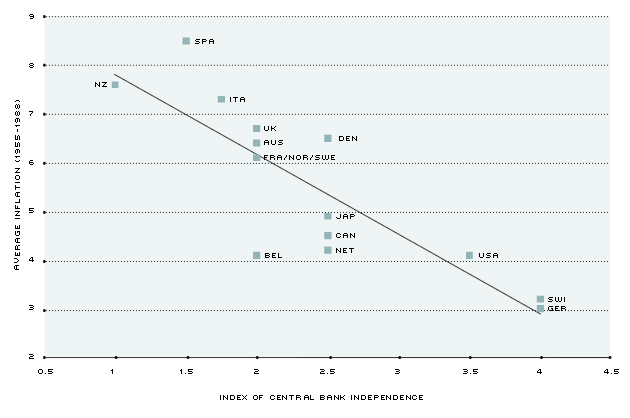
\includegraphics[width=.85\linewidth]{Imagens/paperi1.png}
    \label{fig:fed_independence}
\end{figure}

A Figura~\ref{fig:fmi_independence} ilustra a evolução da média do índice de independência dos bancos centrais (CBI) e das taxas de inflação na América Latina ao longo de um século. Observa-se que, até meados da década de 1990, a região apresentava baixos níveis de independência monetária, acompanhados por inflação elevada e volátil. A partir da segunda metade da década de 1990, com a implementação de reformas institucionais que fortaleceram a autonomia dos bancos centrais, verifica-se uma queda acentuada e sustentada da inflação. Esse movimento indica uma relação inversa clara entre os dois indicadores, corroborando a tese de que a independência institucional contribui para a estabilidade de preços. Os dados reforçam a importância das reformas adotadas na região e estão baseados no estudo de Jácome e Pienknagura (2022) \cite{jacome2022}.

\begin{figure}[H]
    \centering
    \caption{100 anos da independência do banco central e inflação na América Latina}
    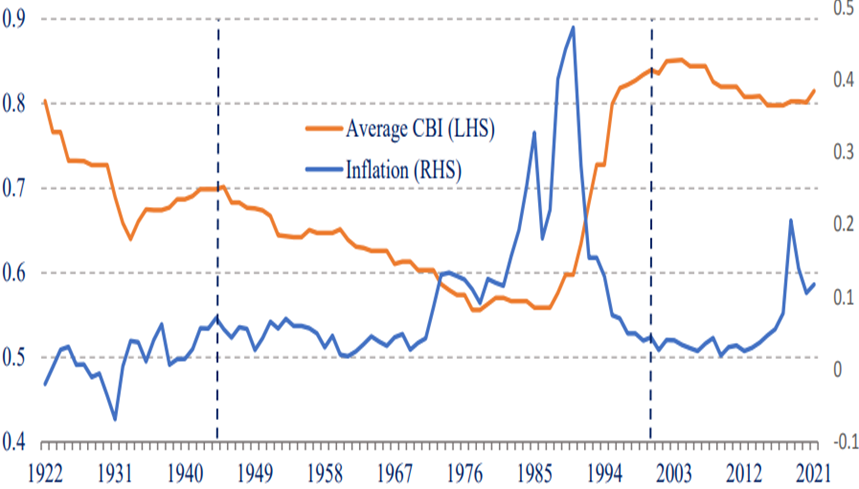
\includegraphics[width=.85\linewidth]{Imagens/paperi2.png}
    \label{fig:fmi_independence}
\end{figure}

A análise das evidências históricas e empíricas evidencia uma relação inversa entre o grau de independência dos bancos centrais e os níveis de inflação. Como mostram dados compilados pelo Federal Reserve Bank of St. Louis (s.d.), países com maior autonomia institucional tendem a apresentar inflação mais baixa e estável \cite{stlouisfed-independencia}. Essa mesma tendência se confirma no caso latino-americano: Jácome e Pienknagura (2022) demonstram que, após a adoção de reformas que ampliaram a independência formal das autoridades monetárias na década de 1990, os países da região experimentaram uma significativa redução da inflação e maior estabilidade macroeconômica \cite{jacome2022}.

Esses resultados sugerem que a autonomia do banco central pode fortalecer a credibilidade das decisões monetárias e ampliar sua eficácia no controle da inflação e na estabilização da economia. No entanto, permanece a questão sobre o quanto essa independência se traduz, de fato, em maior \emph{potência} da política monetária — isto é, em sua capacidade de produzir os efeitos desejados sobre os preços e a atividade econômica real.

Diante desse contexto, este trabalho formula a seguinte \textbf{pergunta de pesquisa}:

\begin{center}
\vspace{0.5em}
\textbf{\Large Como o grau de Independência do Banco Central influencia a Potência da Política Monetária?}
\vspace{0.5em}
\end{center}

\section*{\textbf{Referencial Teórico}}
\addcontentsline{toc}{section}{\textbf{Referencial Teórico}}

\subsection*{\textbf{Teoria Institucional}}
\addcontentsline{toc}{subsection}{\textbf{Teoria Institucional}}

A literatura sobre independência do Banco Central (BC) enfatiza que sua autonomia institucional é um fator decisivo para a eficácia da política monetária. Conforme argumentam Acemoglu et al. (2008), instituições mais independentes são menos vulneráveis à captura política e tendem a produzir melhores resultados macroeconômicos, especialmente em contextos com baixo controle institucional externo \cite{acemoglu2008}. O fluxo ilustrado na Figura~\ref{fig:bc_independente} apresenta o encadeamento lógico pelo qual a independência do BC reduz a interferência política, fortalece sua credibilidade e contribui para a ancoragem das expectativas inflacionárias. Isso, por sua vez, aumenta a potência da política monetária, promovendo maior estabilidade macroeconômica e um ambiente propício ao crescimento. Em contraste, a Figura~\ref{fig:bc_nao_independente} mostra que a ausência de independência gera decisões sujeitas a interesses políticos de curto prazo, comprometendo a credibilidade do BC e resultando em maior volatilidade da inflação. Essa instabilidade compromete a eficácia da política monetária e pode levar ao uso do banco central como instrumento de financiamento do gasto público, com potenciais desequilíbrios fiscais e econômicos. Assim, os esquemas apresentados na Figura~\ref{fig:comparacao_bc} sintetizam visualmente os efeitos teóricos esperados conforme o grau de independência da autoridade monetária, oferecendo uma base conceitual robusta para a análise empírica proposta neste trabalho.

\begin{figure}[H]
    \centering
    \caption{Cenários de condução da política monetária conforme grau de independência}
    \begin{subfigure}[b]{0.45\textwidth}
        \centering
        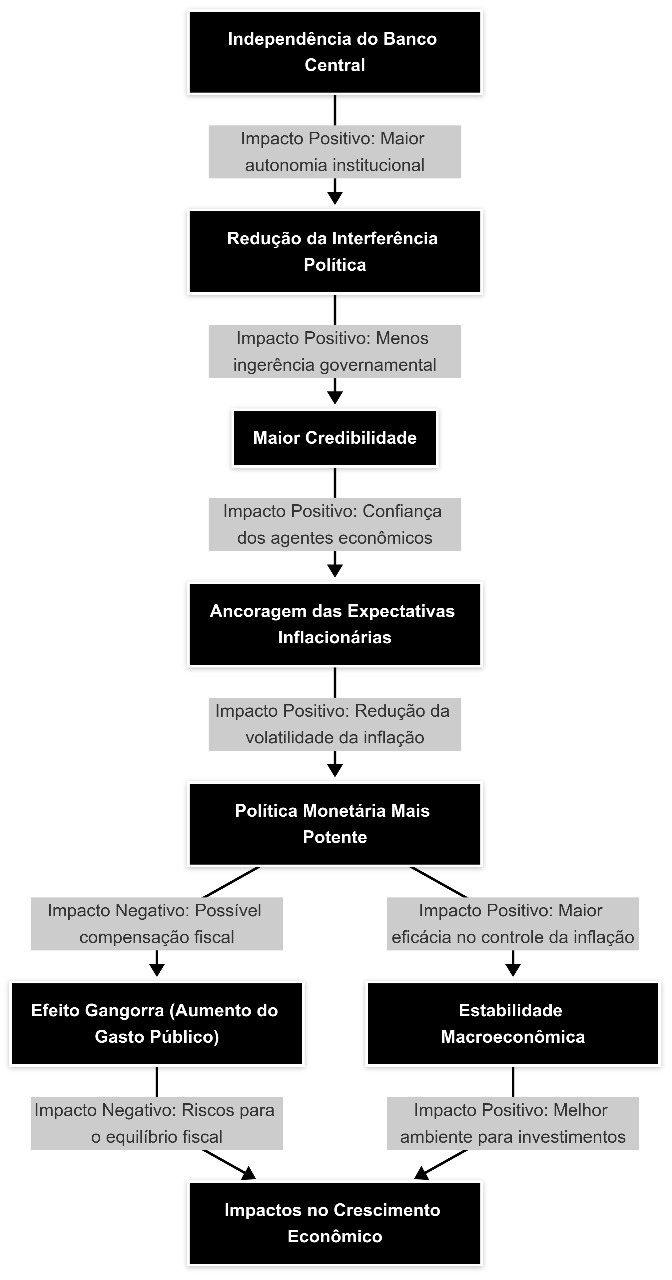
\includegraphics[width=\linewidth]{Imagens/m2i1.jpg}
        \caption{Banco Central Independente}
        \label{fig:bc_independente}
    \end{subfigure}
    \hfill
    \begin{subfigure}[b]{0.45\textwidth}
        \centering
        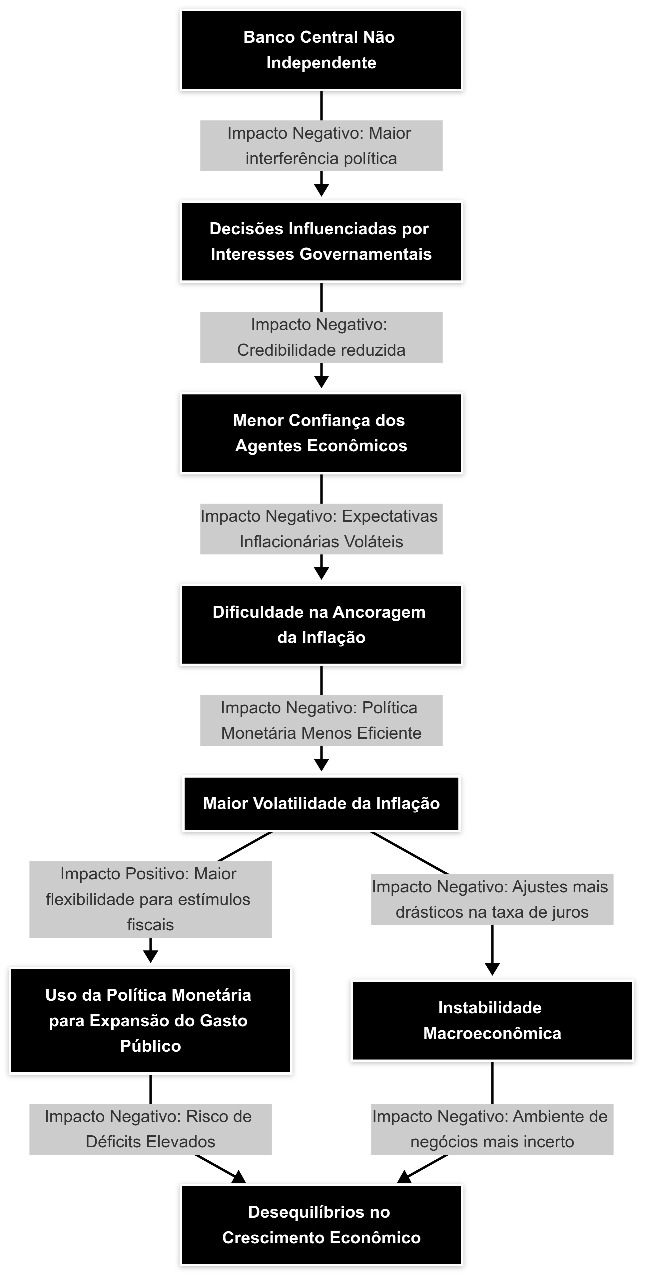
\includegraphics[width=\linewidth]{Imagens/m2i2.jpg}
        \caption{Banco Central Não Independente}
        \label{fig:bc_nao_independente}
    \end{subfigure}
    \label{fig:comparacao_bc}
\end{figure}

Adrian, Khan e Menand (2024) propõem um novo índice de independência dos bancos centrais que visa capturar de maneira mais abrangente os aspectos institucionais envolvidos. O índice vai além da tradicional separação entre independência política e econômica, ao incorporar dimensões como autonomia orçamentária, composição do conselho diretor, estabilidade legal do mandato e autonomia operacional. Utilizando dados legislativos de mais de 180 países, os autores mostram que o novo índice tem maior poder explicativo sobre a estabilidade inflacionária, especialmente em economias emergentes. A proposta representa um avanço metodológico relevante, permitindo comparações mais refinadas entre arranjos institucionais e seus efeitos macroeconômicos \cite{adrian2024}.

Unsal e Papageorgiou (2023) argumentam que a análise da independência dos bancos centrais deve considerar múltiplas dimensões institucionais, indo além da autonomia formal. Os autores propõem uma abordagem baseada em indicadores compostos que incluem accountability, transparência, metas explícitas e estratégias operacionais. Através de um novo banco de dados global e técnicas de análise de componentes principais, demonstram que a eficácia da política monetária depende não apenas da independência legal, mas da coerência entre instrumentos, mandatos e mecanismos de comunicação. Essa perspectiva amplia a compreensão sobre como diferentes estruturas institucionais condicionam os resultados monetários \cite{unsal2023}.

\subsection*{\textbf{Teoria Macroeconômica}}
\addcontentsline{toc}{subsection}{\textbf{Teoria Macroeconômica}}

Jácome e Pienknagura (2022) exploram a relação entre independência do banco central e inflação na América Latina ao longo de um período de mais de cem anos. Utilizando uma abordagem histórica e institucional, os autores mostram que a independência só gera efeitos duradouros sobre a estabilidade de preços quando é sustentada por instituições sólidas e mecanismos de governança confiáveis. Em contextos onde o arcabouço institucional é frágil, a independência formal tende a ser ineficaz ou revertida. Os achados sugerem que reformas legais devem vir acompanhadas de práticas que assegurem o cumprimento dos mandatos e a proteção contra pressões políticas de curto prazo \cite{jacome2022}.

Para analisar a relação entre \textbf{independência do Banco Central} e \textbf{política monetária}, é útil adotar um \emph{modelo Novo-Keynesiano} como estrutura básica, pois este tipo de modelo enfatiza a importância das \emph{expectativas} e da \emph{consistência temporal} na determinação dos níveis de inflação e produto. Na essência, o modelo contempla duas equações principais: a \textbf{Curva de Phillips Novo-Keynesiana} e a \textbf{Equação IS}, que descrevem, respectivamente, a evolução da inflação e a dinâmica da demanda agregada.

A Curva de Phillips Novo-Keynesiana (NKPC) descreve a dinâmica da inflação em função das expectativas e do hiato do produto. Sua formulação básica é:

\begin{equation}
\pi_t = \beta \, E_t[\pi_{t+1}] + \kappa \, (y_t - y_t^*) + \epsilon_t,
\label{eq:nkpc}
\end{equation}

\noindent onde $\pi_t$ representa a inflação no período $t$, $E_t[\pi_{t+1}]$ são as expectativas racionais da inflação futura, $(y_t - y_t^*)$ é o hiato do produto, $\beta$ é o fator de desconto intertemporal, $\kappa$ reflete a rigidez nominal e $\epsilon_t$ é um choque de oferta. A literatura mostra que a credibilidade do Banco Central (BC), associada ao seu grau de independência, afeta diretamente $E_t[\pi_{t+1}]$, tornando-se fundamental para o controle da inflação \cite{unsal2023, gali2015}.

Do lado da demanda, a equação IS é usada para modelar o desvio do produto como função da taxa de juros real e das expectativas:

\begin{equation}
y_t - y_t^* = E_t[y_{t+1} - y_{t+1}^*] - \phi \big( i_t - E_t[\pi_{t+1}] - r_t^* \big) + \eta_t,
\label{eq:is}
\end{equation}

\noindent onde $i_t$ é a taxa de juros nominal, $r_t^*$ é a taxa de juros real de equilíbrio e $\eta_t$ representa choques de demanda. O parâmetro $\phi$ mede a sensibilidade da demanda às variações da taxa de juros real. Essa estrutura permite compreender como o grau de autonomia do BC afeta sua capacidade de estabilizar a economia por meio da política monetária.

A Regra de Taylor fornece um arcabouço para descrever como o BC ajusta sua taxa de juros diante de desvios da inflação e do produto:

\begin{equation}
i_t = \rho \, i_{t-1} + (1 - \rho) \big[ r_t^* + \pi_t + \alpha (\pi_t - \pi^*) + \gamma (y_t - y_t^*) \big] + \nu_t,
\label{eq:taylor}
\end{equation}

\noindent em que $\pi^*$ é a meta de inflação, $\nu_t$ é um choque de política monetária, e $\rho$ representa o grau de suavização na resposta da taxa de juros. Os parâmetros $\alpha$ e $\gamma$ indicam a intensidade da resposta à inflação e ao hiato do produto, respectivamente. Quando o BC é independente, espera-se que ele utilize essa regra com maior rigor técnico e menor influência política, aumentando a credibilidade do regime monetário \cite{adrian2024, woodford2003, unsal2023, gali2015}.

Para formalizar o papel da independência, considera-se a função de perda do BC:

\begin{equation}
\mathcal{L} = \sum_{t=0}^{\infty} \beta^t \left[ (\pi_t - \pi^*)^2 + \lambda (y_t - y_t^*)^2 \right],
\label{eq:loss_function}
\end{equation}

\noindent onde $\lambda$ representa o peso atribuído à estabilização do produto. A presença de independência fortalece o compromisso com a estabilidade de preços, minimizando a influência de objetivos políticos de curto prazo. Entretanto, a literatura mostra que a independência formal nem sempre se traduz em independência efetiva. Estudos como \cite{jacome2022, acemoglu2008} indicam que, na ausência de instituições sólidas, a autonomia legal pode ser revertida, comprometendo a eficácia da política monetária.

O modelo também enfatiza o papel da ancoragem das expectativas de inflação. Considerando:

\begin{equation}
\pi_t^E = \chi \pi^T + (1 - \chi)\pi_{t-1},
\label{eq:expectations}
\end{equation}

\noindent onde $\chi$ mede o grau de ancoragem das expectativas em relação à meta $\pi^T$. Quanto mais próximo de 1, mais confiáveis são as expectativas. Substituindo na Curva de Phillips:

\begin{equation}
\pi_t = \pi_t^E + \alpha (y_t - y^e),
\label{eq:anchored_phillips}
\end{equation}

\noindent mostra-se que a persistência da inflação depende diretamente da capacidade do BC de ancorar expectativas, atributo associado à sua credibilidade institucional.

Adicionalmente, o peso que o BC atribui ao controle da inflação pode ser modelado como dependente do grau de independência:

\begin{equation}
L = (y_t - y^T)^2 + \beta(CBI) \cdot (\pi_t - \pi^T)^2,
\label{eq:loss_beta}
\end{equation}

Mostra o trade-off entre estabilizar a inflação e estabilizar o produto. 

\begin{equation}
\beta(CBI) = \beta_0 + \beta_1 \cdot CBI, \quad \beta_1 > 0,
\label{eq:beta_function}
\end{equation}

\noindent onde $CBI$ é o índice de independência. Com base na minimização dessa função, deriva-se a reação ótima da política monetária:

\begin{equation}
y_t - y^T = - \alpha \cdot \beta(CBI) \cdot (\pi_t - \pi^T),
\label{eq:optimal_response}
\end{equation}

\noindent Essa equação mostra que um BC mais independente responde de forma mais forte a desvios inflacionários, ajustando a atividade econômica de forma mais firme.

Ao incorporar essa equação na Curva IS:

\begin{equation}
y_t = \bar{a} - \sigma (r_t - r^n),
\label{eq:curve_is}
\end{equation}

\noindent obtém-se uma função de reação da taxa de juros:

\begin{equation}
r_t = r^n + \frac{1}{\sigma}(\bar{a} - y^T + \alpha \beta(CBI)(\pi_t - \pi^T)),
\label{eq:reaction_function}
\end{equation}

\noindent De onde se extrai uma versão implícita da Regra de Taylor, com o coeficiente de reação da taxa de juros à inflação:

\begin{equation}
\phi_\pi = \frac{\alpha \cdot \beta(CBI)}{\sigma},
\label{eq:phi_pi}
\end{equation}

\noindent ou seja, quanto maior a independência do BC, maior a resposta da taxa de juros à inflação.

Por fim, a potência da política monetária pode ser definida como:

\begin{equation}
\text{Potência} = \left| \frac{\partial \pi_t}{\partial r_t} \right| = \frac{\sigma}{\alpha \cdot \beta(CBI)},
\label{eq:potencia}
\end{equation}

\noindent indicando que um BC mais independente, ao atribuir maior peso à estabilidade de preços, reduz a sensibilidade da inflação à taxa de juros, mas aumenta a credibilidade e eficácia da política, consolidando sua potência de forma qualitativa e duradoura.

\begin{figure}[H]
    \centering
    \caption{Derivação da teoria econômica}
    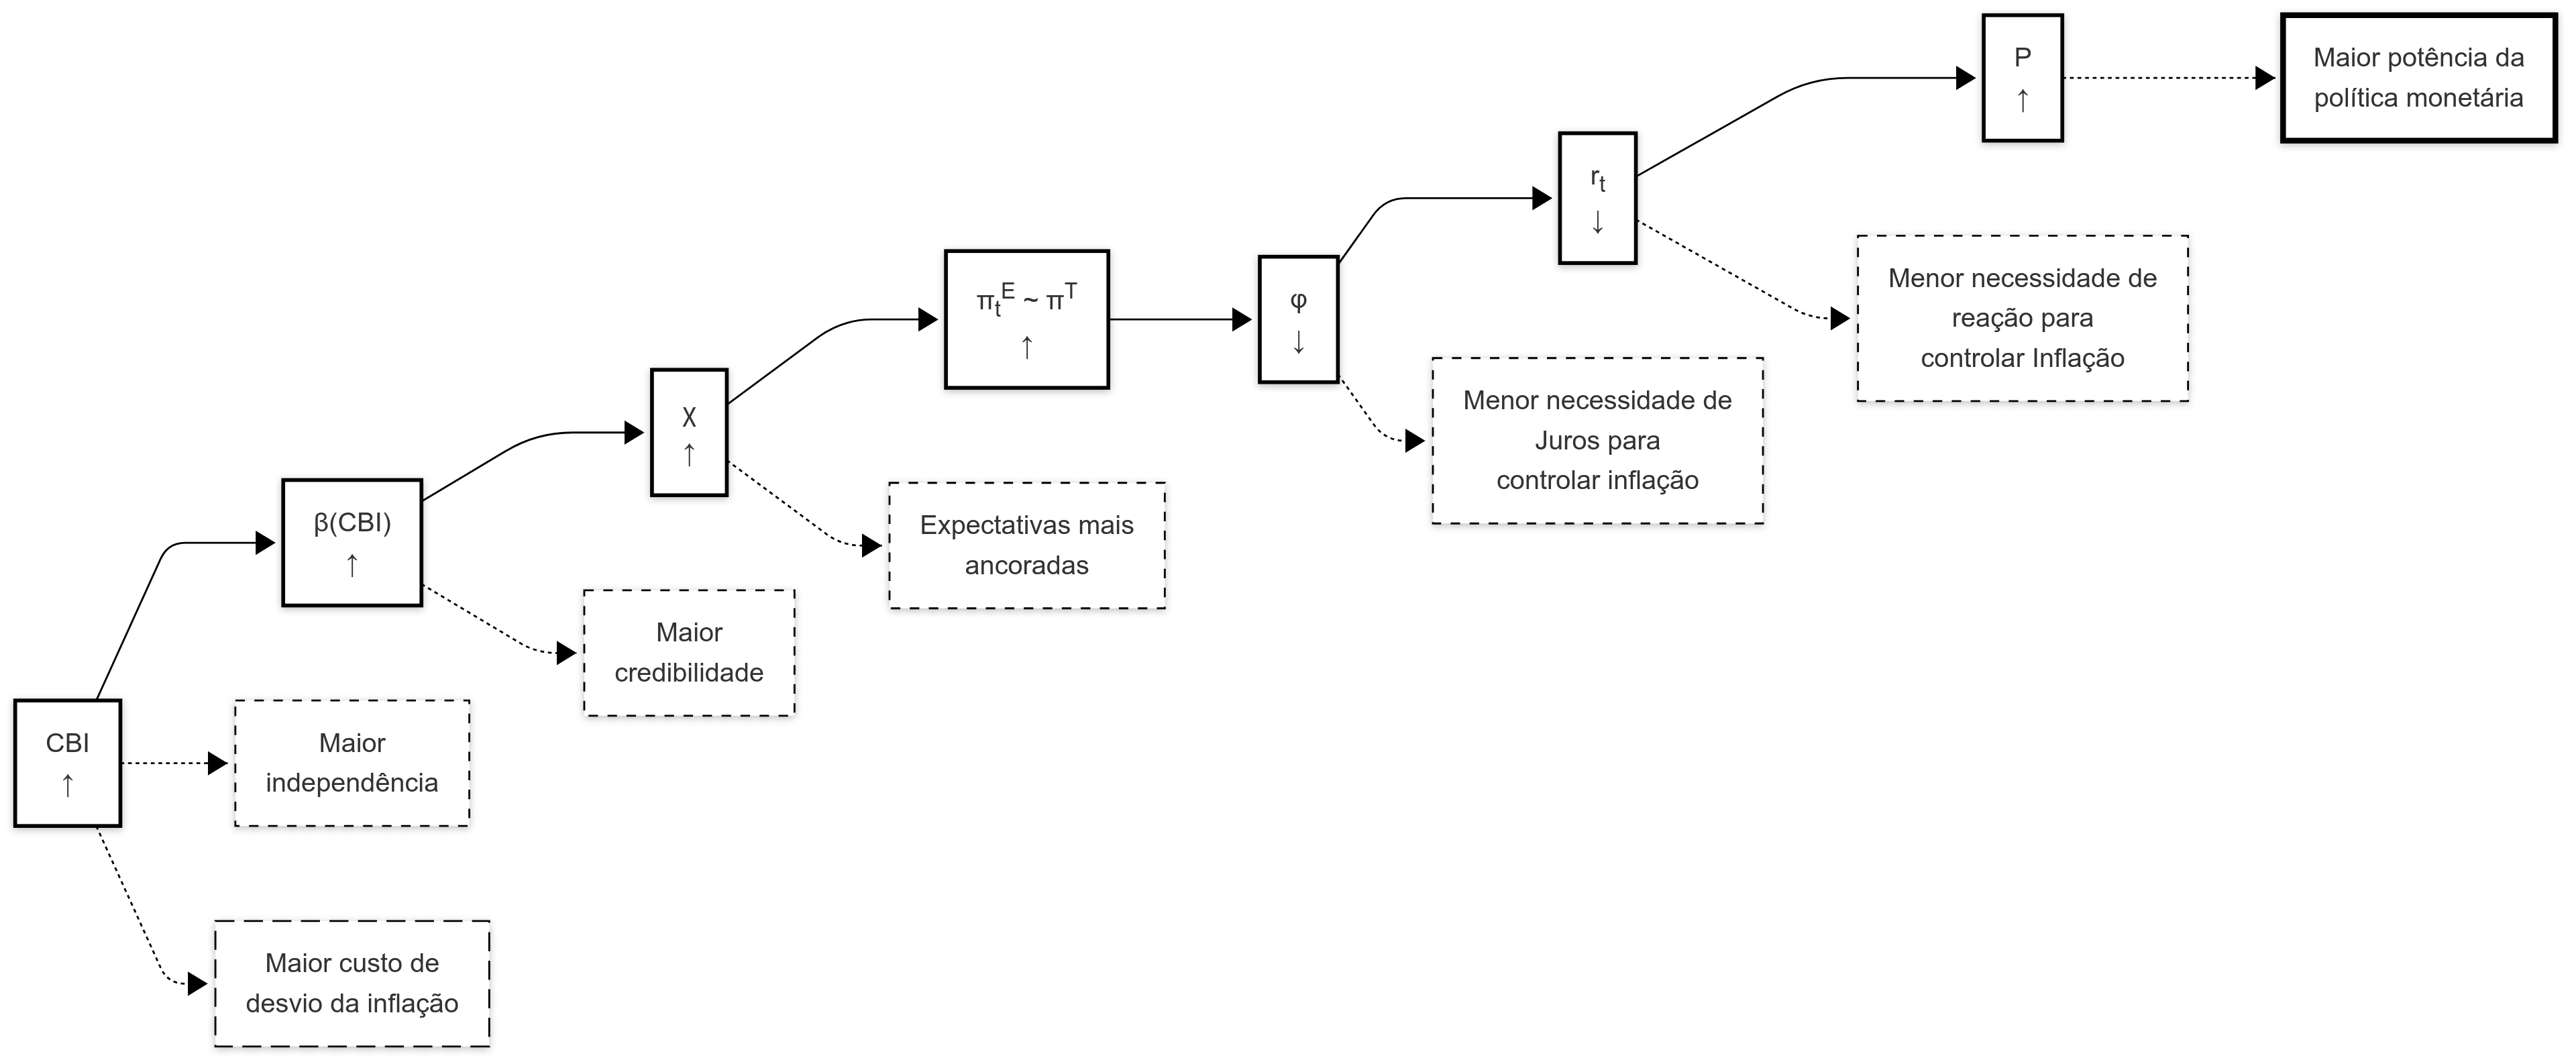
\includegraphics[width=.85\linewidth]{Imagens/paperi3.png}
    \label{fig:intuição_econômica}
\end{figure}

\begin{center}
\vspace{0.5em}
\textbf{\Large Quanto maior o grau de independência do Banco Central, maior será a potência da política monetária no controle inflacionário}
\vspace{0.5em}
\end{center}

A hipótese central propõe que, quanto maior o grau de independência do Banco Central (BC), maior será a potência da política monetária no controle inflacionário. Em outras palavras, a autonomia institucional do BC permite decisões mais técnicas, previsíveis e menos suscetíveis a pressões políticas, fortalecendo sua capacidade de conduzir a inflação para a meta com maior eficácia e menor custo em termos de produto.

Essa hipótese se desdobra em três frentes principais. A primeira diz respeito ao \textbf{efeito sobre a inflação e sua volatilidade}. Espera-se que BCs independentes apresentem menor nível médio de inflação e maior estabilidade, uma vez que operam com credibilidade reforçada e horizonte de planejamento de longo prazo. Isso reduz a necessidade de políticas monetárias reativas e abruptas.

A segunda frente está relacionada à \textbf{ancoragem de expectativas}. A independência fortalece o compromisso do BC com o regime de metas de inflação, contribuindo para o alinhamento das expectativas dos agentes econômicos com a trajetória esperada da inflação. Com isso, as respostas da política monetária se tornam mais eficientes, já que menores desvios exigem menores ajustes na taxa básica de juros.

Por fim, considera-se a \textbf{interação com restrições institucionais}. A literatura aponta que a eficácia da independência formal pode ser limitada em contextos de fragilidade fiscal, instabilidade política ou ausência de mecanismos de governança eficazes. Nesses casos, observa-se o chamado \emph{efeito gangorra}, em que o esforço do BC em conter a inflação pode ser contrabalançado por pressões fiscais expansionistas, comprometendo o impacto líquido da política monetária.

O estudo empírico visa testar essa hipótese avaliando como o grau de independência influencia a capacidade do Banco Central de alinhar a inflação à meta em diferentes países e contextos institucionais. O objetivo é verificar se a autonomia se traduz, na prática, em maior potência monetária — isto é, em uma resposta mais eficaz da inflação aos instrumentos de política disponíveis.


\section*{\textbf{Metodologia}}
\addcontentsline{toc}{section}{\textbf{Metodologia}}

\subsection*{\textbf{Base de Dados}}
\addcontentsline{toc}{subsection}{\textbf{Base de Dados}}

A base de dados utilizada neste estudo foi construída a partir da integração de diversas fontes, com ênfase nos dados provenientes do Fundo Monetário Internacional (FMI), do World Development Indicators (WDI) ,do CBIdata, do The Global Economy, Eiko(LSEG) e MacroBond. As bases foram coletadas e organizadas para permitir uma análise econômica e institucional aprofundada de múltiplos países ao longo do tempo.

Os dados macroeconômicos essenciais foram extraídos utilizando duas importantes bibliotecas do R:
\begin{itemize}
    \item \textbf{World Development Indicators (WDI)}: Através da biblioteca \texttt{WDI} \cite{WDI}, foram baixadas séries históricas de variáveis fundamentais, tais como o Produto Interno Bruto (PIB) Real, inflação e dívida, iniciando em 1960. Esse processo envolveu o uso dos pacotes \texttt{tidyverse} \cite{tidyverse} e \texttt{countrycode} \cite{countrycode} para filtrar e padronizar os dados, excluindo agrupamentos regionais que não eram pertinentes à análise. Fonte: \url{https://data.worldbank.org/indicator}.
    \item \textbf{Fundo Monetário Internacional (FMI)}: Utilizando a biblioteca \texttt{imf.data} \cite{imf.data}, foram obtidas séries históricas referentes à política monetária, como as taxas de juros dos bancos centrais, com dados disponíveis em periodicidade anual para o período de 1960 a 2025. Ressalta-se que o FMI funciona como um repositório de dados originalmente reportados por fontes nacionais e internacionais. Fonte: \url{https://data.imf.org}.
\end{itemize}

A base do CBIdata foi construída a partir de uma planilha em Excel que contém os índices de independência dos bancos centrais, fundamentais para mensurar a autonomia das instituições monetárias em relação ao governo. Esses índices, que incluem o índice CBIE de Romelli (2022, 2024) e os índices clássicos de Grilli, Masciandaro e Tabellini (1991) e de Cukierman, Webb e Neyapti (1992), foram extraídos de legislações e documentos oficiais dos bancos centrais. Para a importação desta planilha, foi utilizada a biblioteca \texttt{readxl} \cite{readxl}. Essa fonte permite explorar a relação entre a independência dos bancos centrais e as principais variáveis macroeconômicas, como inflação e crescimento econômico. Fonte: \url{https://cbidata.org/}.

A base \texttt{InflationForecast (FMI)} foi extraída do site \texttt{TheGlobalEconomy.com}, que agrega projeções de inflação calculadas pelo FMI. As expectativas de inflação são fundamentais para o modelo ecônomico, dado que na Curva de Phillips Novo-Keynesiana (NKPC) ela é um componente fundamental para formulação da inflação. Fonte: \url{https://www.theglobaleconomy.com/}. 

A base \texttt{taget(Eikon)} e \textit{taget(MacroBond)} agregametas de inflação divulgadas pelos Bancos Centrais de cada país |(que tem meta de inflação). As metas de inflação são fundamentais para o modelo ecônomico, dado que na Curva de Phillips Novo-Keynesiana (NKPC) ela é um componente fundamental para formulação da inflação. 

Essa abordagem integrada, com o uso extensivo das bibliotecas \texttt{WDI} \cite{WDI} e \texttt{imf.data} \cite{imf.data} para a extração e padronização dos dados, e a elaboração cuidadosa do dataframe de metas de inflação, possibilitou a criação de uma base robusta e detalhada. Tal base é capaz de sustentar análises comparativas entre diferentes períodos e regiões, contribuindo para uma compreensão mais aprofundada das dinâmicas econômicas e institucionais dos países analisados.

A amostra consiste em um \textbf{painel país–ano} cobrindo \textbf{78 países}, no período de \textbf{2000 a 2023}. Essa estrutura permite analisar, simultaneamente, variações \emph{entre} países (por exemplo, diferentes graus de independência do banco central – \emph{CBI}) e \emph{ao longo do tempo} dentro de cada país.

\begin{figure}[H]
    \centering
    \caption{Cobertura de Dados por País e Variável}
    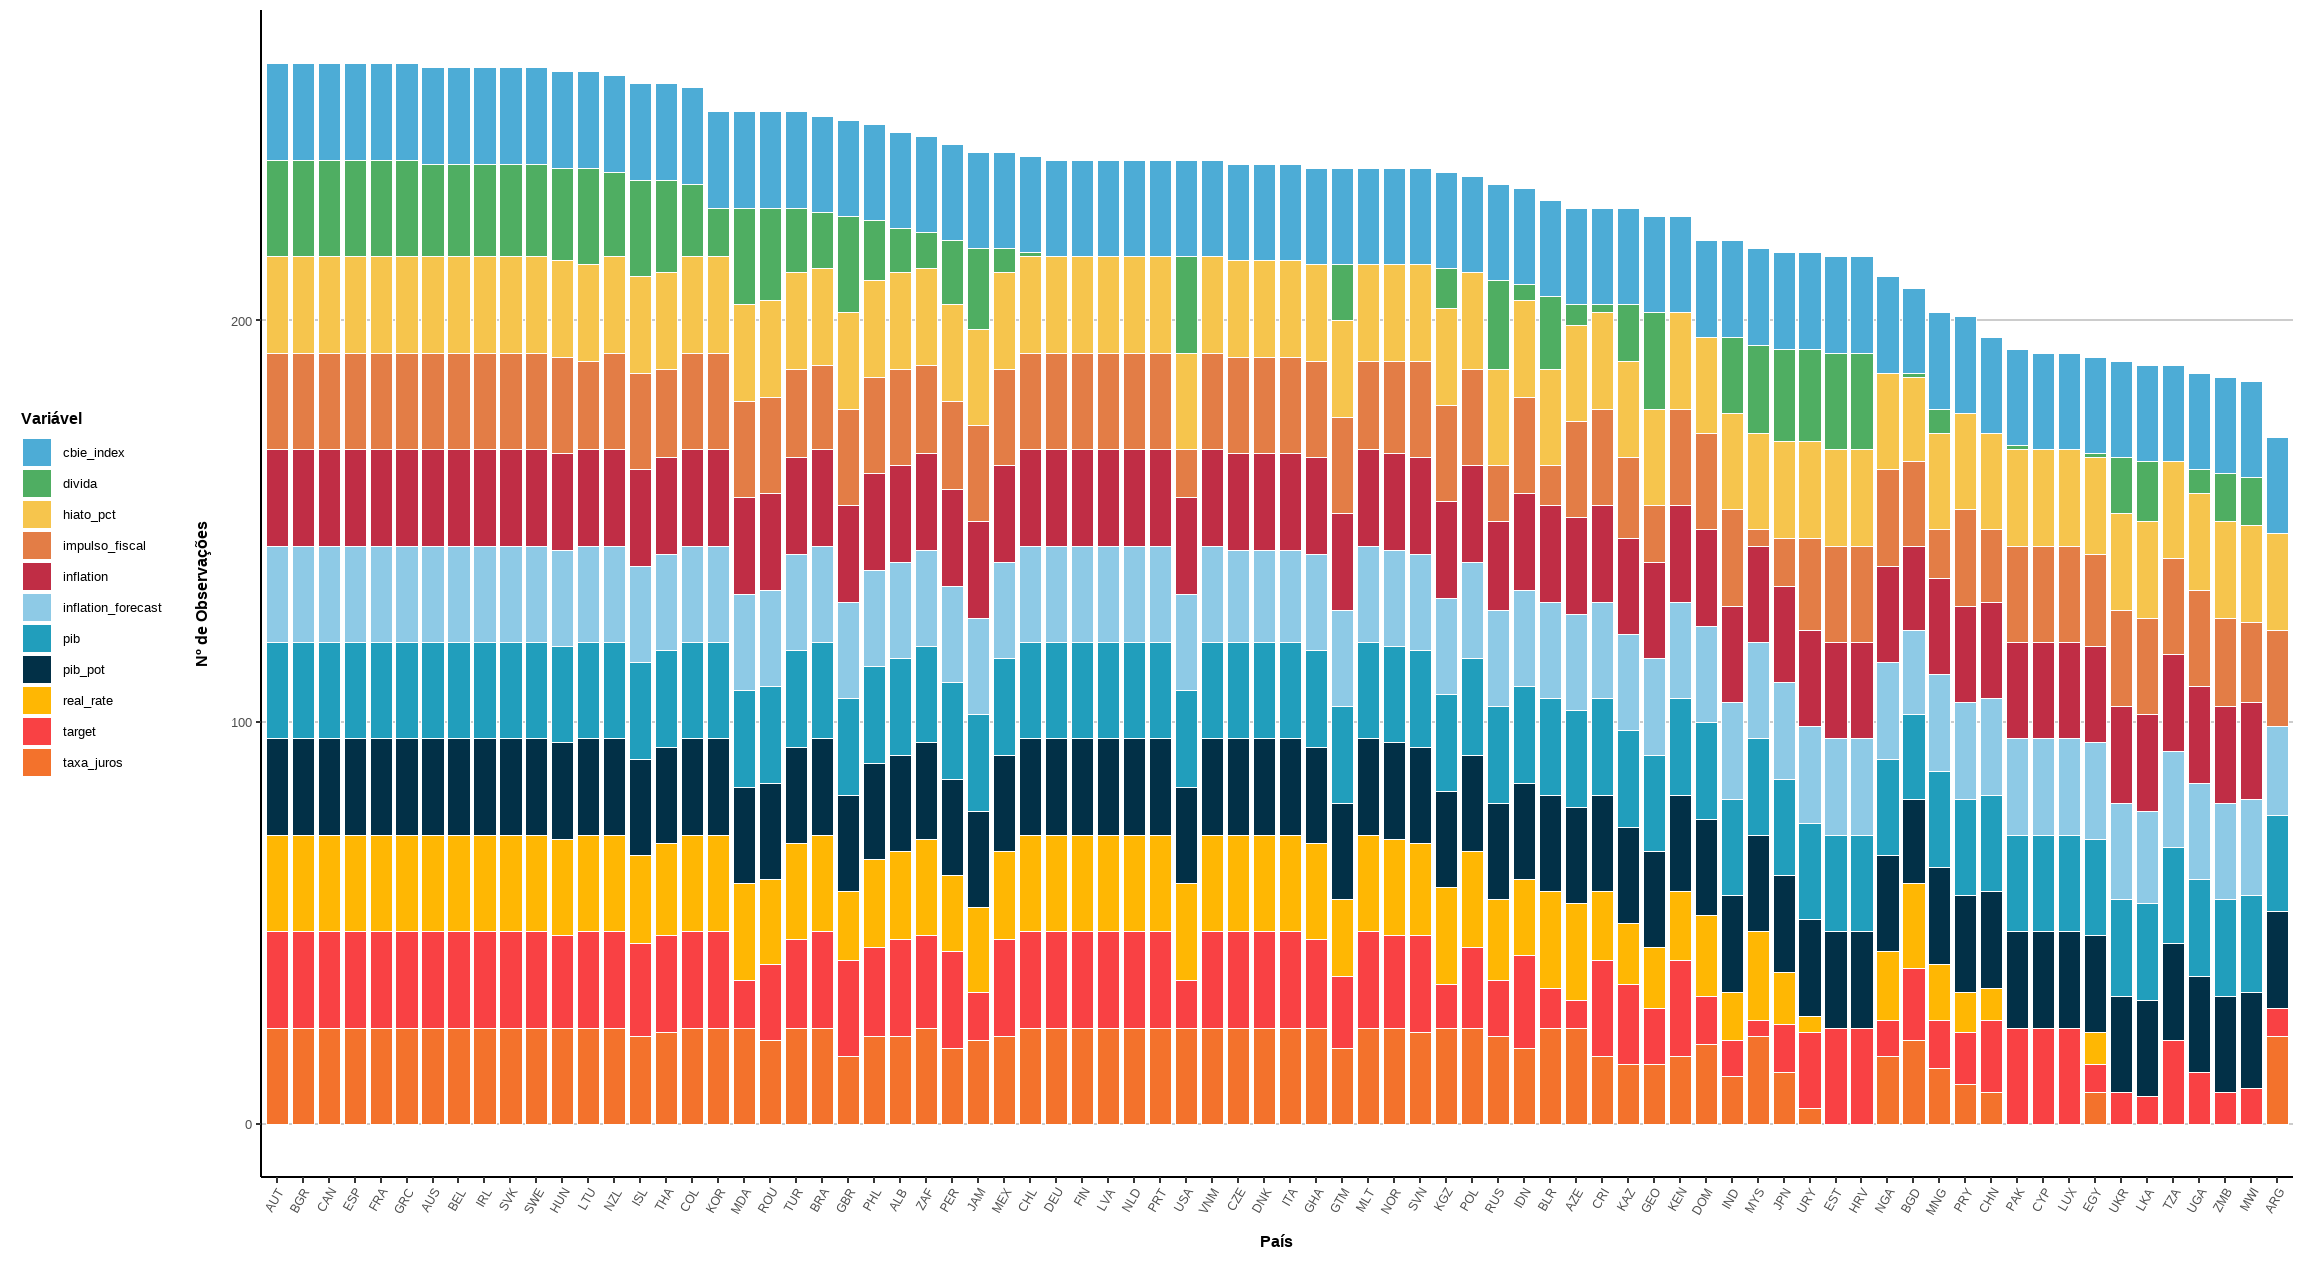
\includegraphics[width=.85\linewidth]{Imagens/paperi4.png}
    \label{fig:observações_absolutas}

    \footnotesize{Fonte: Elaborado pelos autores | WDI + FMI + CBIE}
\end{figure}

\begin{figure}[H]
    \centering
    \caption{Proporção de dados observados por país (2000–2023)}
    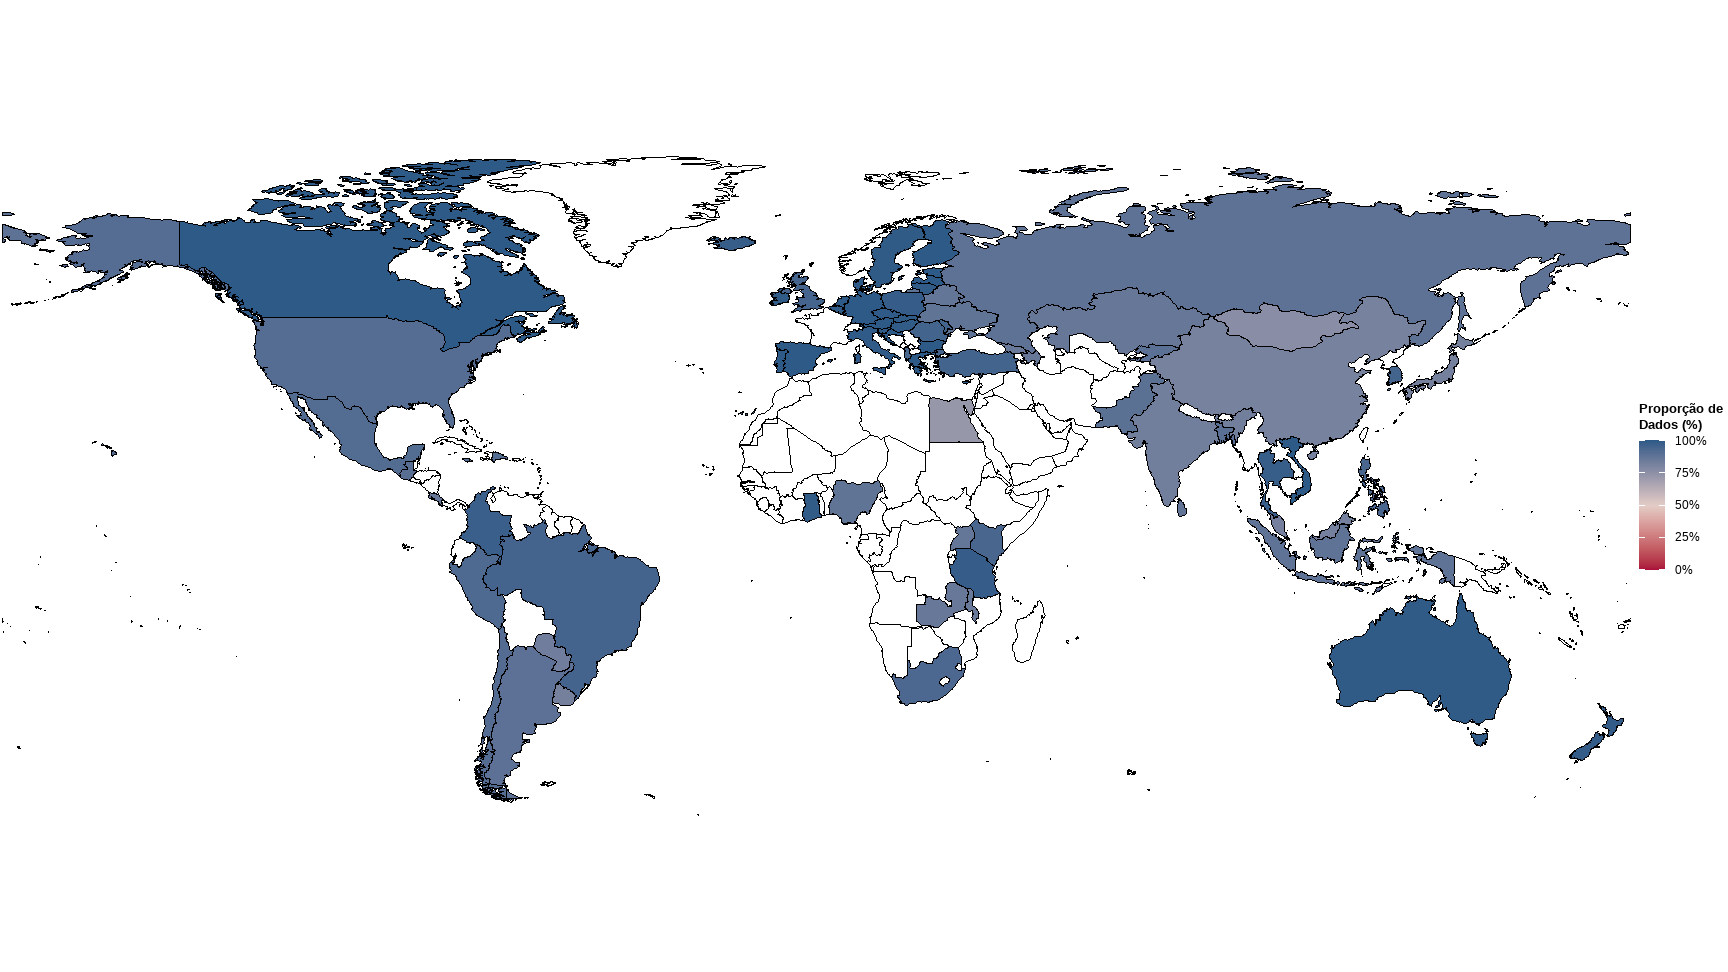
\includegraphics[width=.85\linewidth]{Imagens/paperi5.png}
    \label{fig:observações_relativas}

    \footnotesize{Fonte: Elaborado pelos autores | WDI + FMI + CBIE}
\end{figure}

Ao realizar uma análise inicial em relação às figuras 5 e 6, pode-se reforçar importantes elementos sobre a base de dados utilizada. É possível observar que o CBI Index apresenta ampla cobertura entre os países da amostra, o que justifica sua inclusão como variável central no modelo empírico. Em contrapartida, identificam-se lacunas significativas nas séries de dívida pública e taxa de juros, o que exige o uso de métodos robustos (como o estimador System-GMM) para lidar com a natureza desbalanceada do painel.

Além disso, a distribuição geográfica da amostra, evidenciada no mapa global da Figura 6, mostra que todas as regiões do FMI estão representadas, mitigando potenciais vieses de seleção e fortalecendo a validade externa das inferências obtidas. 

\begin{table}[H]
\centering
\caption{Descrição e origem das variáveis utilizadas na análise econométrica.}
\renewcommand{\arraystretch}{1.3}
\setlength{\tabcolsep}{4pt}
\small
\begin{tabular}{>{\normalfont}l>{\normalfont}l>{\normalfont}p{7cm}}
\toprule
\rowcolor[HTML]{F2F5F9}
\textbf{Variável} & \textbf{Origem} & \textbf{Descrição} \\
\midrule
País & WDI & Nome do país \\
\rowcolor[HTML]{F9FBFD}
Ano & WDI / FMI / CBIE & Ano da observação \\
PIB & WDI & Produto Interno Bruto nominal (USD correntes) \\
\rowcolor[HTML]{F9FBFD}
Inflação & WDI & Inflação anual observada (\%) \\
Expectativa de Inflação & TheGlobalEconomy & Expectativa de inflação (\%) \\
\rowcolor[HTML]{F9FBFD}
Taxa de Juros Nominal & FMI & Taxa de juros nominal do banco central (\%) \\
Independência do BC & CBIdata & Índice de independência do Banco Central [0,1] \\
\rowcolor[HTML]{F9FBFD}
Independência do BC (PM) & CBIdata & Índice de independência da Política Monetária [0,1] \\
Independência do BC (PM-Q1) & CBIdata & Resposta dada à forma de Política Monetária [0,1] \\
\rowcolor[HTML]{F9FBFD}
Dívida & WDI & Dívida pública bruta (\% do PIB) \\
Meta de Inflação & LSEG + Macrobond & Meta inflacionária (\%) \\
\rowcolor[HTML]{F9FBFD}
Impulso Fiscal & FMI & Impulso fiscal: - (Déficit/Superávit Primário (t) - Déficit/Superávit Primário (t-1) (\% PIB)) \\
\rowcolor[HTML]{F9FBFD}
PIB Potencial & Construída & Estimativa do PIB potencial (Filtro HP) \\
Gap Inflacionário & Construída & Inflação - Meta (p.p) \\
\rowcolor[HTML]{F9FBFD}
Hiato do Produto & Construída & Hiato do produto (\%): \\
Taxa de Juros Real & Construída & Taxa de juros real (\%): \\
\bottomrule
\end{tabular}
\label{tab:base_dados}
\vspace{.1cm}
\footnotesize{
Nota: \textbf{WDI} = World Development Indicators (Banco Mundial); 
\textbf{FMI} = Fundo Monetário Internacional; 
\textbf{CBIdata} = Central Bank Independence database; 
\textbf{HP} = Hodrick–Prescott; 
\textbf{LSEG} = London Stock Exchange Group.
}
\end{table}

\begin{table}[H]
\centering
\small
\caption{Completude das variáveis da base (máx.\ = 1869 observações)}
\setlength{\tabcolsep}{3pt}
\begin{tabular}{lcccccccc}
\toprule
\textbf{Variável} & \textbf{PIB} & \textbf{Inflação} & \textbf{Inf.\ Esp.} & \textbf{Meta} & \textbf{Juros} & \textbf{Dívida} & \textbf{Imp.\ Fisc.} & \textbf{CBI} \\
\midrule
Total possível           & 1869 & 1869 & 1869 & 1869 & 1869 & 1869 & 1869 & 1869 \\
Observações presentes    & 1869 & 1843 & 1863 & 1516 & 1419 & \;923 & 1745 & 1869 \\
Países 100\% completos  & 78   & 76   & 73   & 40   & 39   & 14   & 57   & 78   \\
Países parciais          & 0    & 1    & 5    & 38   & 28   & 41   & 21   & 0    \\
Países sem dados         & 0    & 1    & 0    & 0    & 11   & 23   & 0    & 0    \\
\bottomrule
\multicolumn{9}{l}{\footnotesize Fonte: WDI, IMF‑IFS, TheGlobalEconomy, Eikon, MacroBond.}
\end{tabular}
\label{tab:observações_base_dados}
\end{table}


\subsection*{\textbf{Análise Descritiva}}
\addcontentsline{toc}{subsection}{\textbf{Análise Descritiva}}

\begin{figure}[H]
    \centering
    \caption{Evolução da inflação média por grupos de independência}
    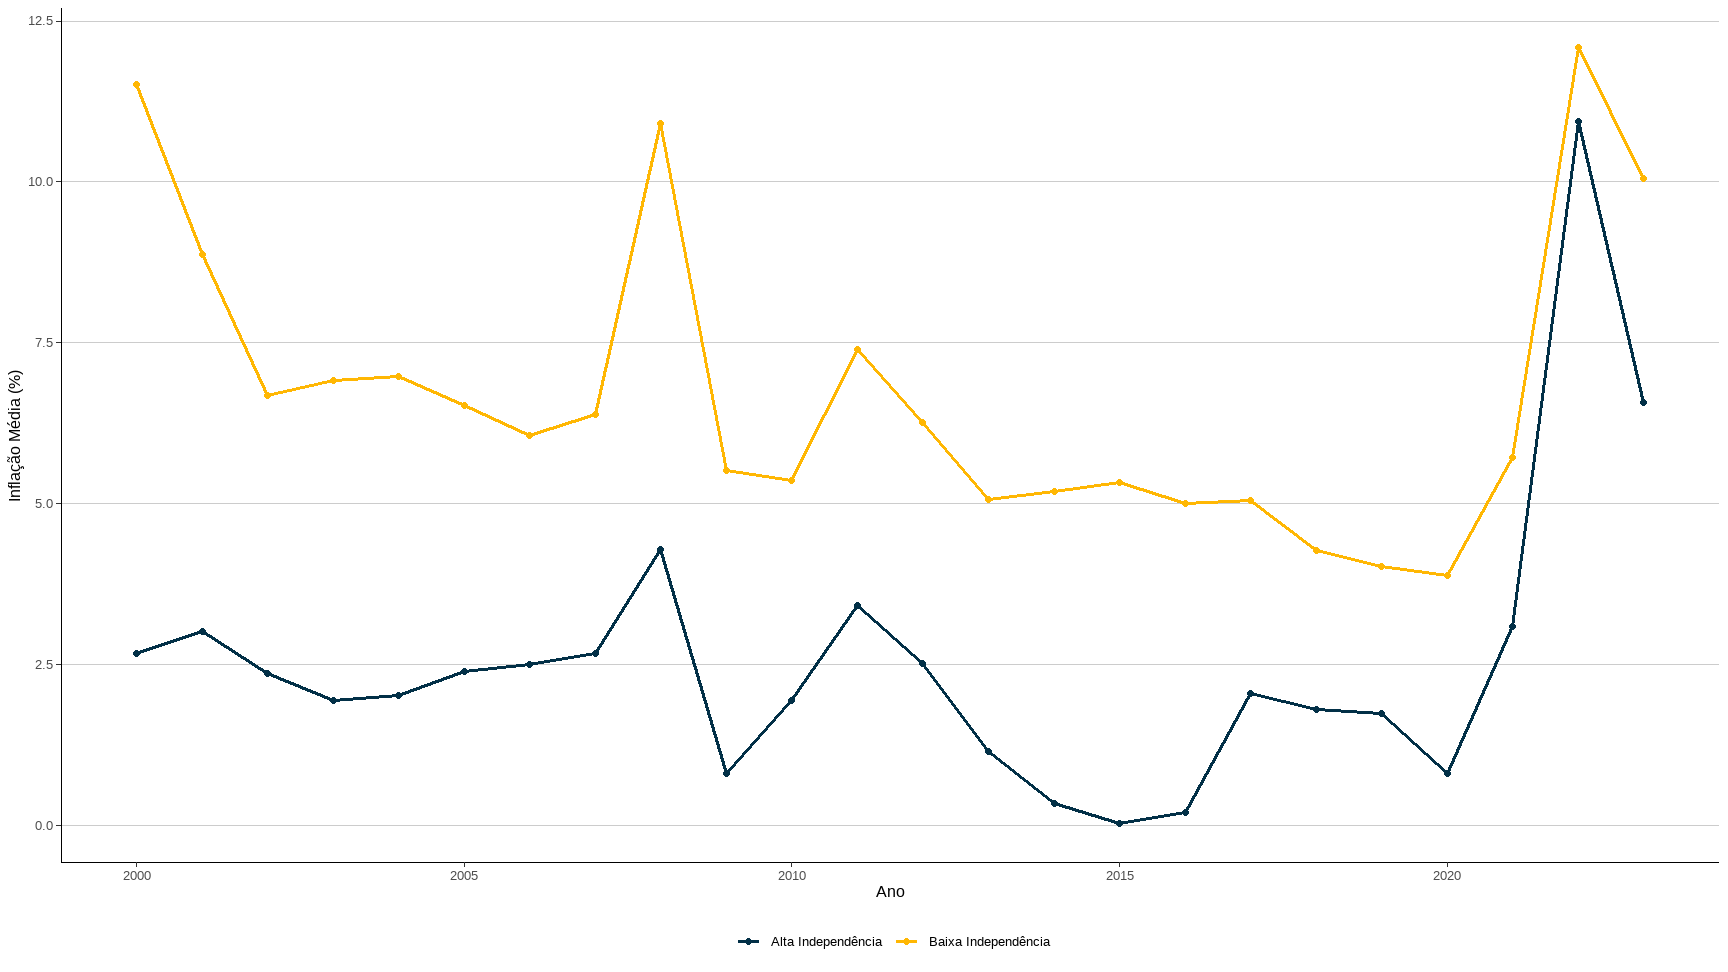
\includegraphics[width=.85\linewidth]{Imagens/paperi6.png}
    \label{fig:infl_media}

    \footnotesize{Fonte: Elaborado pelos autores | WDI + FMI + CBIE}
\end{figure}

Os países situados no quartil superior do índice de independência apresentam inflação média persistentemente menor ao longo de todo o período, enquanto o grupo menos independente exibe um \textit{patamar} bem mais elevado e volátil.  
A distância entre as duas trajetórias estreita‑se gradualmente até 2014, mas volta a crescer após o choque inflacionário de 2021–22: a inflação dispara em ambos os grupos, porém a alta é muito mais intensa onde a independência é baixa.  

O resultado sugere que a credibilidade própria de bancos centrais mais autônomos torna o processo desinflacionário menos custoso, reforçando a hipótese de maior potência da política monetária nesses regimes.

\begin{figure}[H]
    \centering
    \caption{Evolução do gap de inflação média por grupos de independência}
    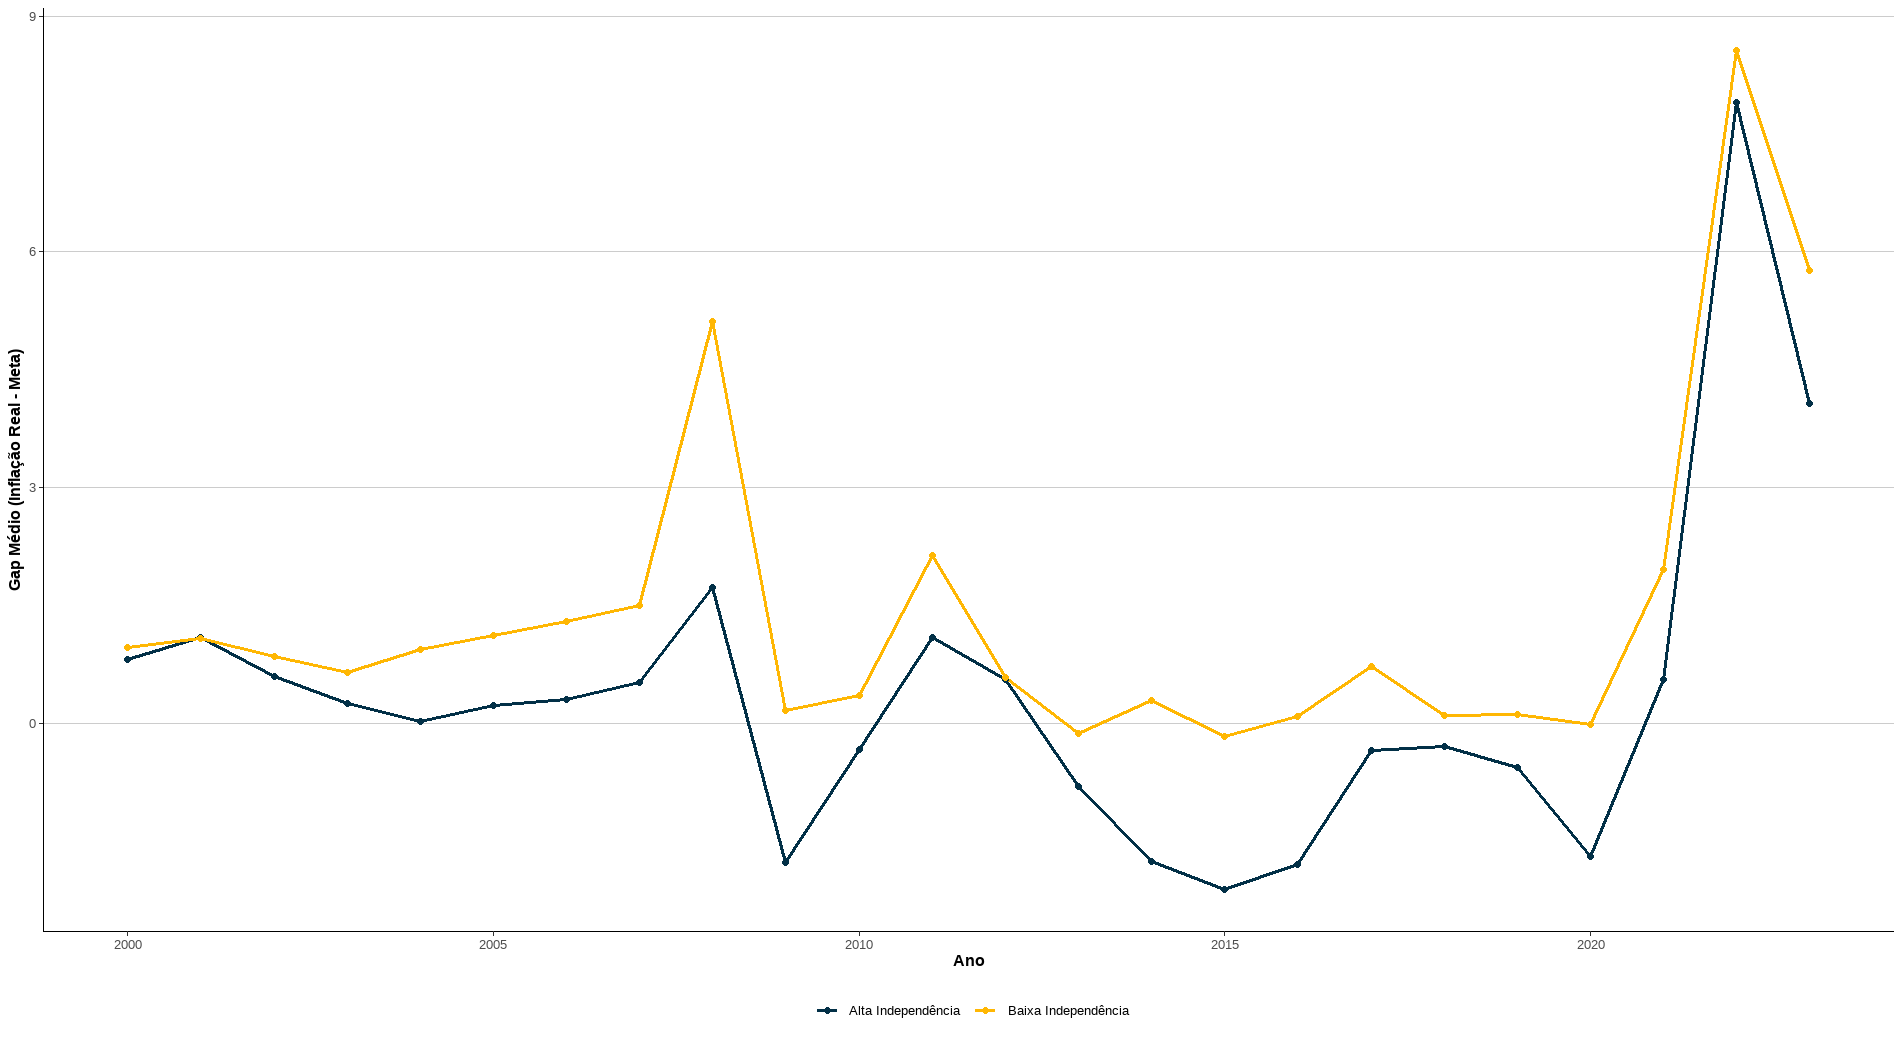
\includegraphics[width=.85\linewidth]{Imagens/paperi10.png}
    \label{fig:gap_media}

    \footnotesize{Fonte: Elaborado pelos autores | WDI + FMI + CBIE}
\end{figure}

O desvio frente à meta (inflação real menos meta) é sistematicamente menor — e, em vários anos, negativo — nos países mais independentes, sinalizando \textit{overshooting} limitado ou mesmo abaixo da meta.  
Nos países menos independentes, o gap é positivo em praticamente todo o intervalo, com picos em 2008 e 2022.  
A divergência reforça que um banco central autônomo suaviza choques através de expectativas mais ancoradas, reduzindo a magnitude do ajuste necessário na taxa de juros.

\begin{figure}[H]
    \centering
    \caption{Gap inflacionário médio e \(\pm1\sigma\) por decil de CBI}
    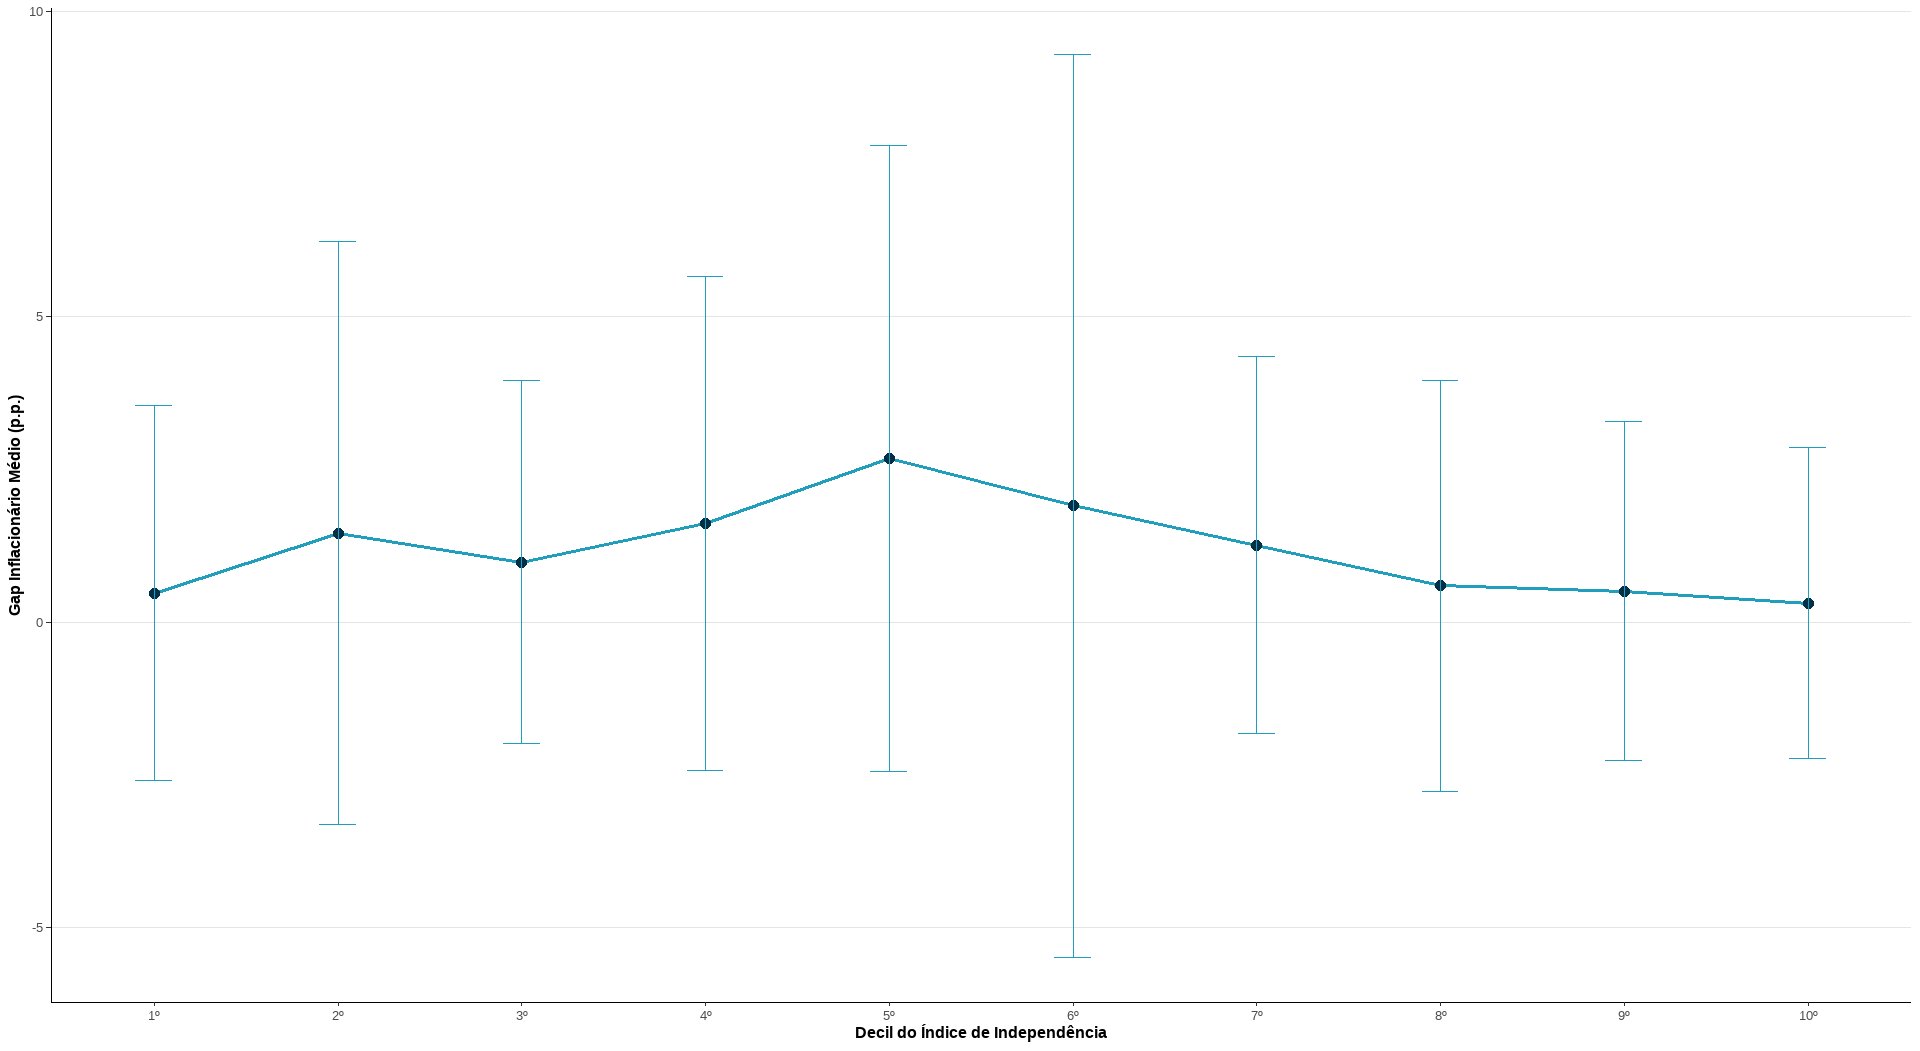
\includegraphics[width=.85\linewidth]{Imagens/paperi7.png}
    \label{fig:decil_gap}

    \footnotesize{Fonte: Elaborado pelos autores | WDI + FMI + CBIE}
\end{figure}

O gap inflacionário cresce dos 1º aos 5º décis, atinge o pico e passa a cair nos décis superiores, aproximando‑se de zero quando o CBI supera 80\%.  
Além disso, a dispersão (barras de \(\pm1\sigma\)) diminui nos últimos décis, indicando menor incerteza inflacionária onde a independência é elevada.  
O formato em “U invertido” sugere retornos marginais decrescentes: ganhos iniciais de independência ainda não são suficientes para reduzir o gap, mas níveis altos produzem ancoragem efetiva das expectativas.

\begin{figure}[H]
    \centering
    \caption{Evolução anual do índice de independência (CBI)}
    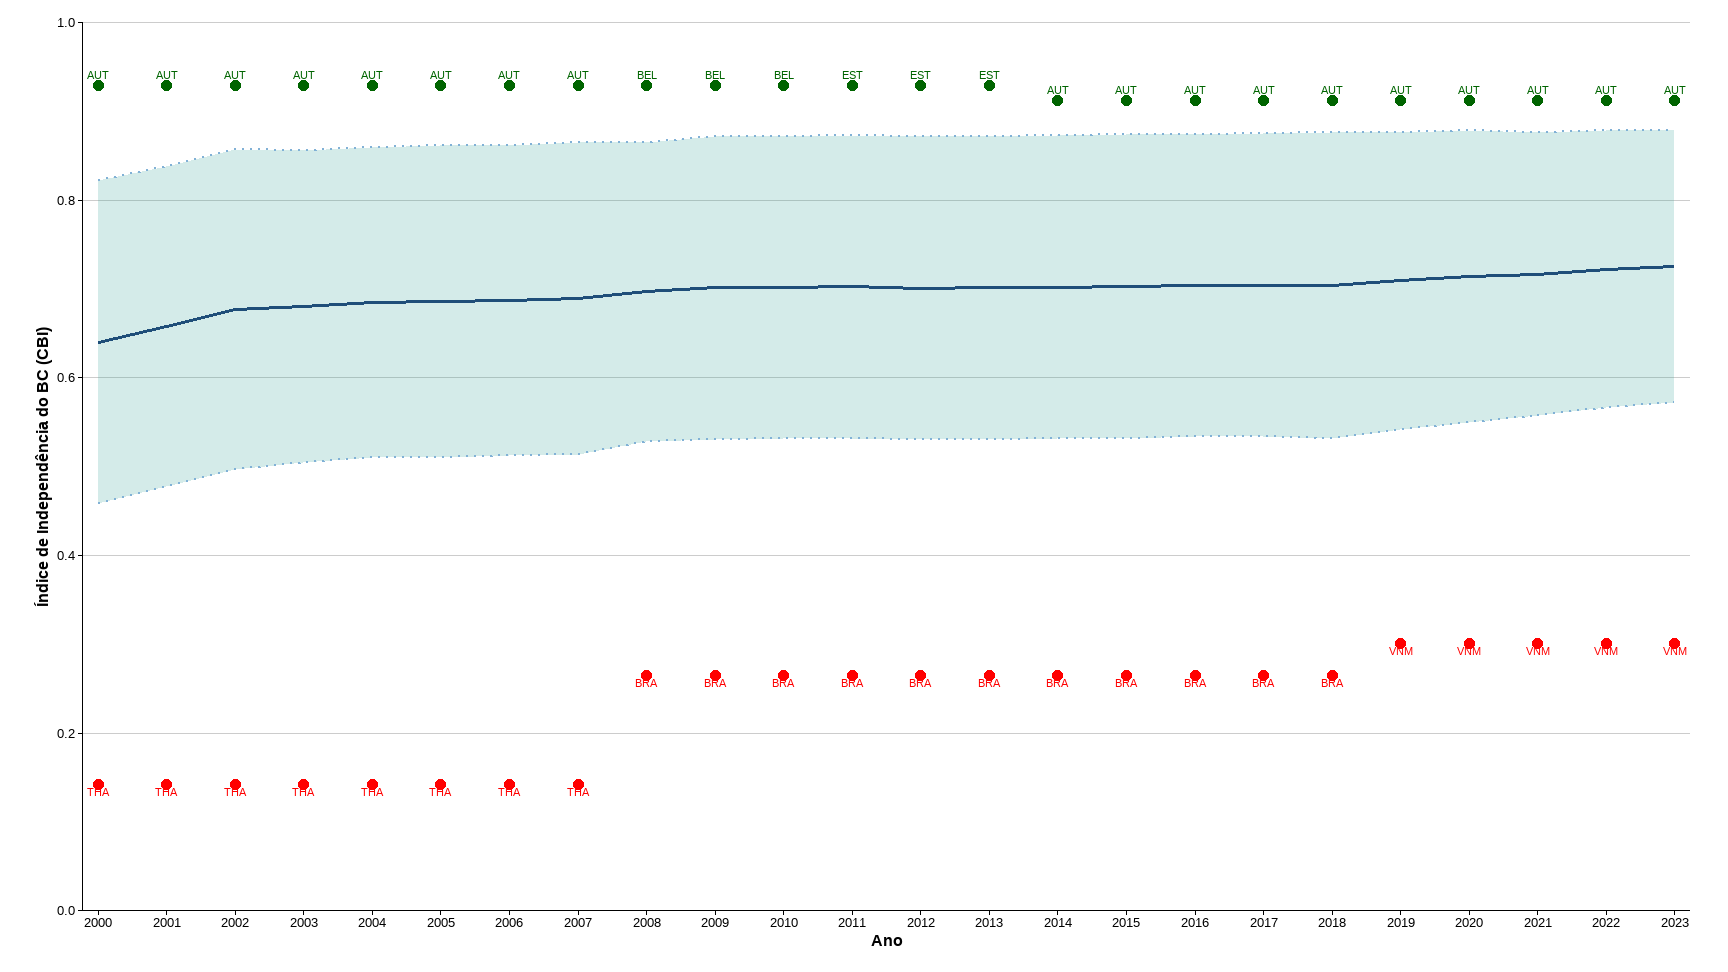
\includegraphics[width=.85\linewidth]{Imagens/paperi8.png}
    \label{fig:cbi_trend}

    \footnotesize{Fonte: Elaborado pelos autores | WDI + FMI + CBIE}
\end{figure}

A média global do CBI sobe cerca de 0,05 ponto entre 2000 e 2023, refletindo reformas institucionais graduais.  
Outliers positivos (Áustria, Bélgica, Estónia) permanecem próximos de 1, ao passo que o grupo de menor independência (Tailândia, Vietnã) estagna abaixo de 0,3.  
A banda de \(\pm1\sigma\) estreita‑se até 2010 e volta a alargar após 2018, indicando heterogeneidade renovada nas práticas de governança monetária.

\begin{figure}[H]
    \centering
    \caption{Trajetória média global de CBI, gap, inflação e juro real}
    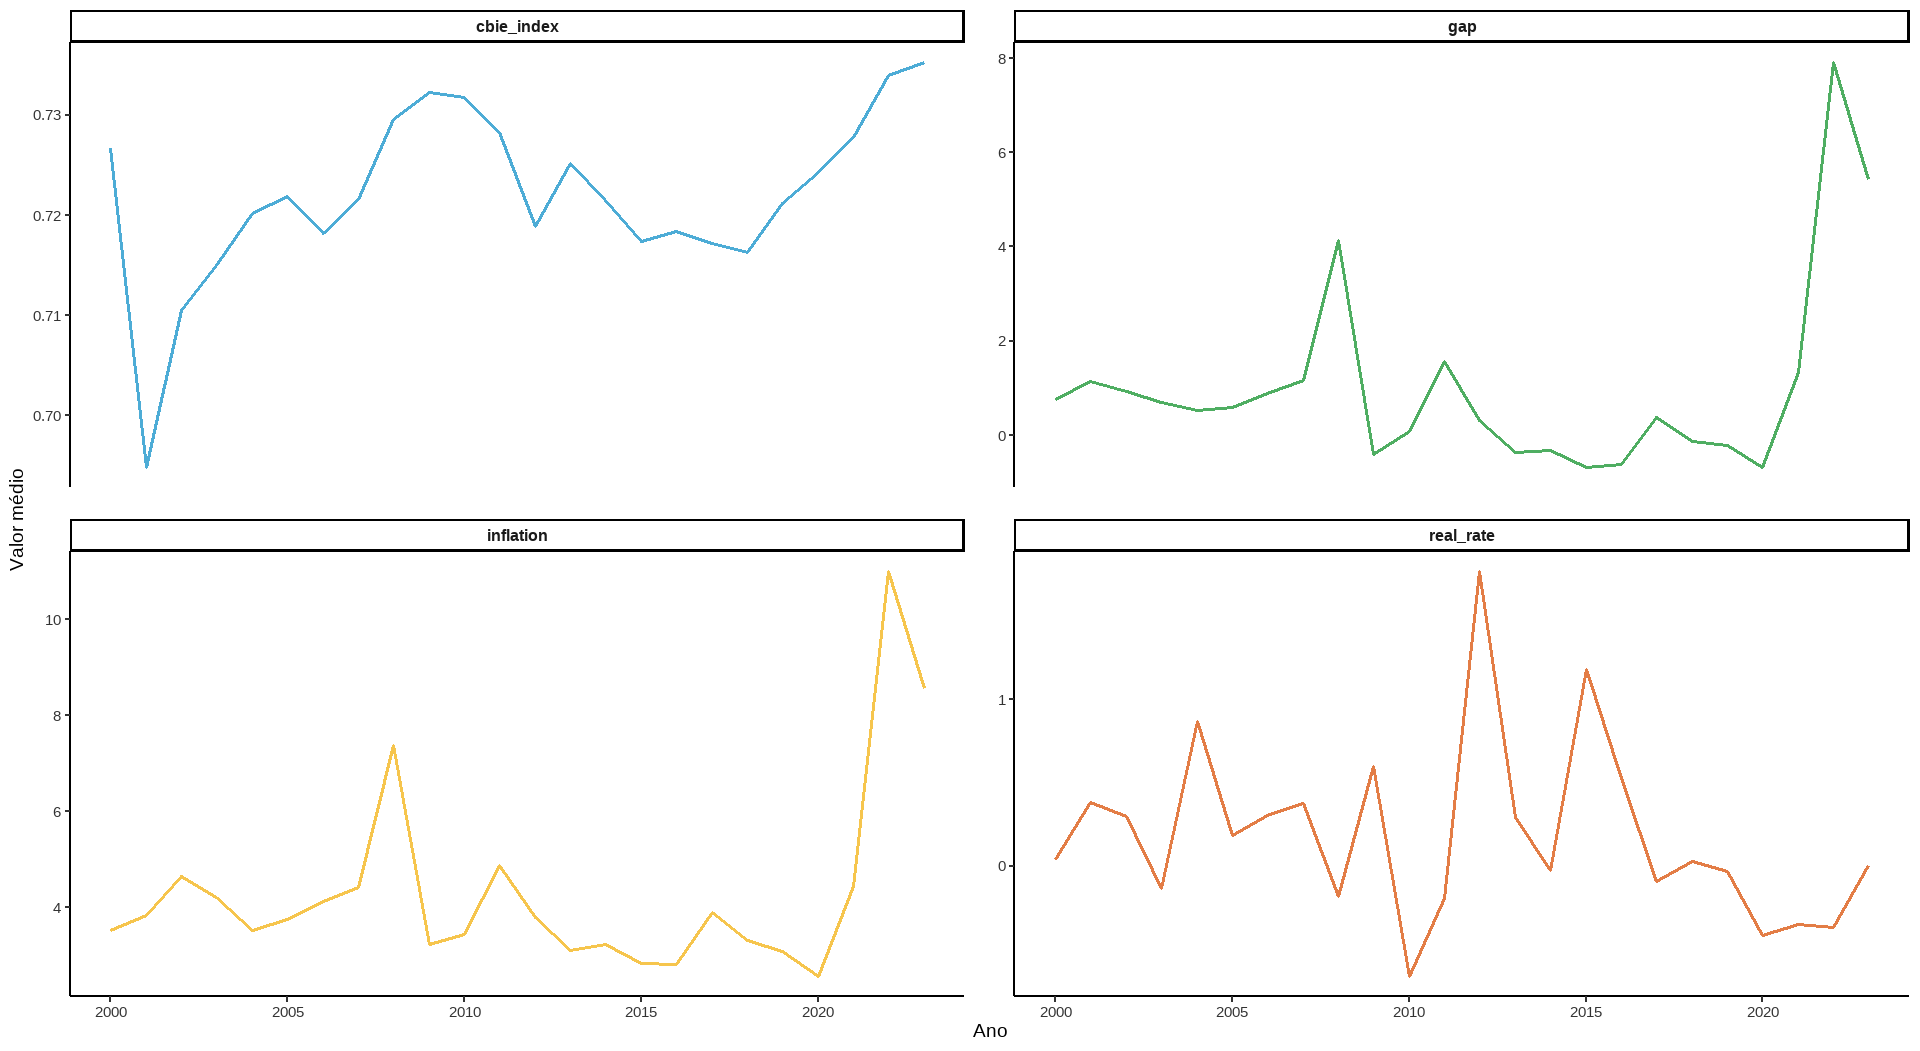
\includegraphics[width=.85\linewidth]{Imagens/paperi9.png}
    \label{fig:series_painel}

    \footnotesize{Fonte: Elaborado pelos autores | WDI + FMI + CBIE}
\end{figure}

O CBI cresce suavemente, enquanto o \textit{gap} e a inflação exibem picos coincidentes (2008, 2022).  
O juro real salta em 2011–13 — reação de política contracíclica a pressões de preços — e volta a subir em 2022, mas com menor amplitude onde o CBI é mais alto (vide Fig.~\ref{fig:gap_media}).  
A co‑movimentação sugere que credibilidade reduz a necessidade de ajustes agressivos na taxa real de juros para estabilizar preços.

\begin{figure}[H]
    \centering
    \caption{Independência do BC e volatilidade condicional do gap}
    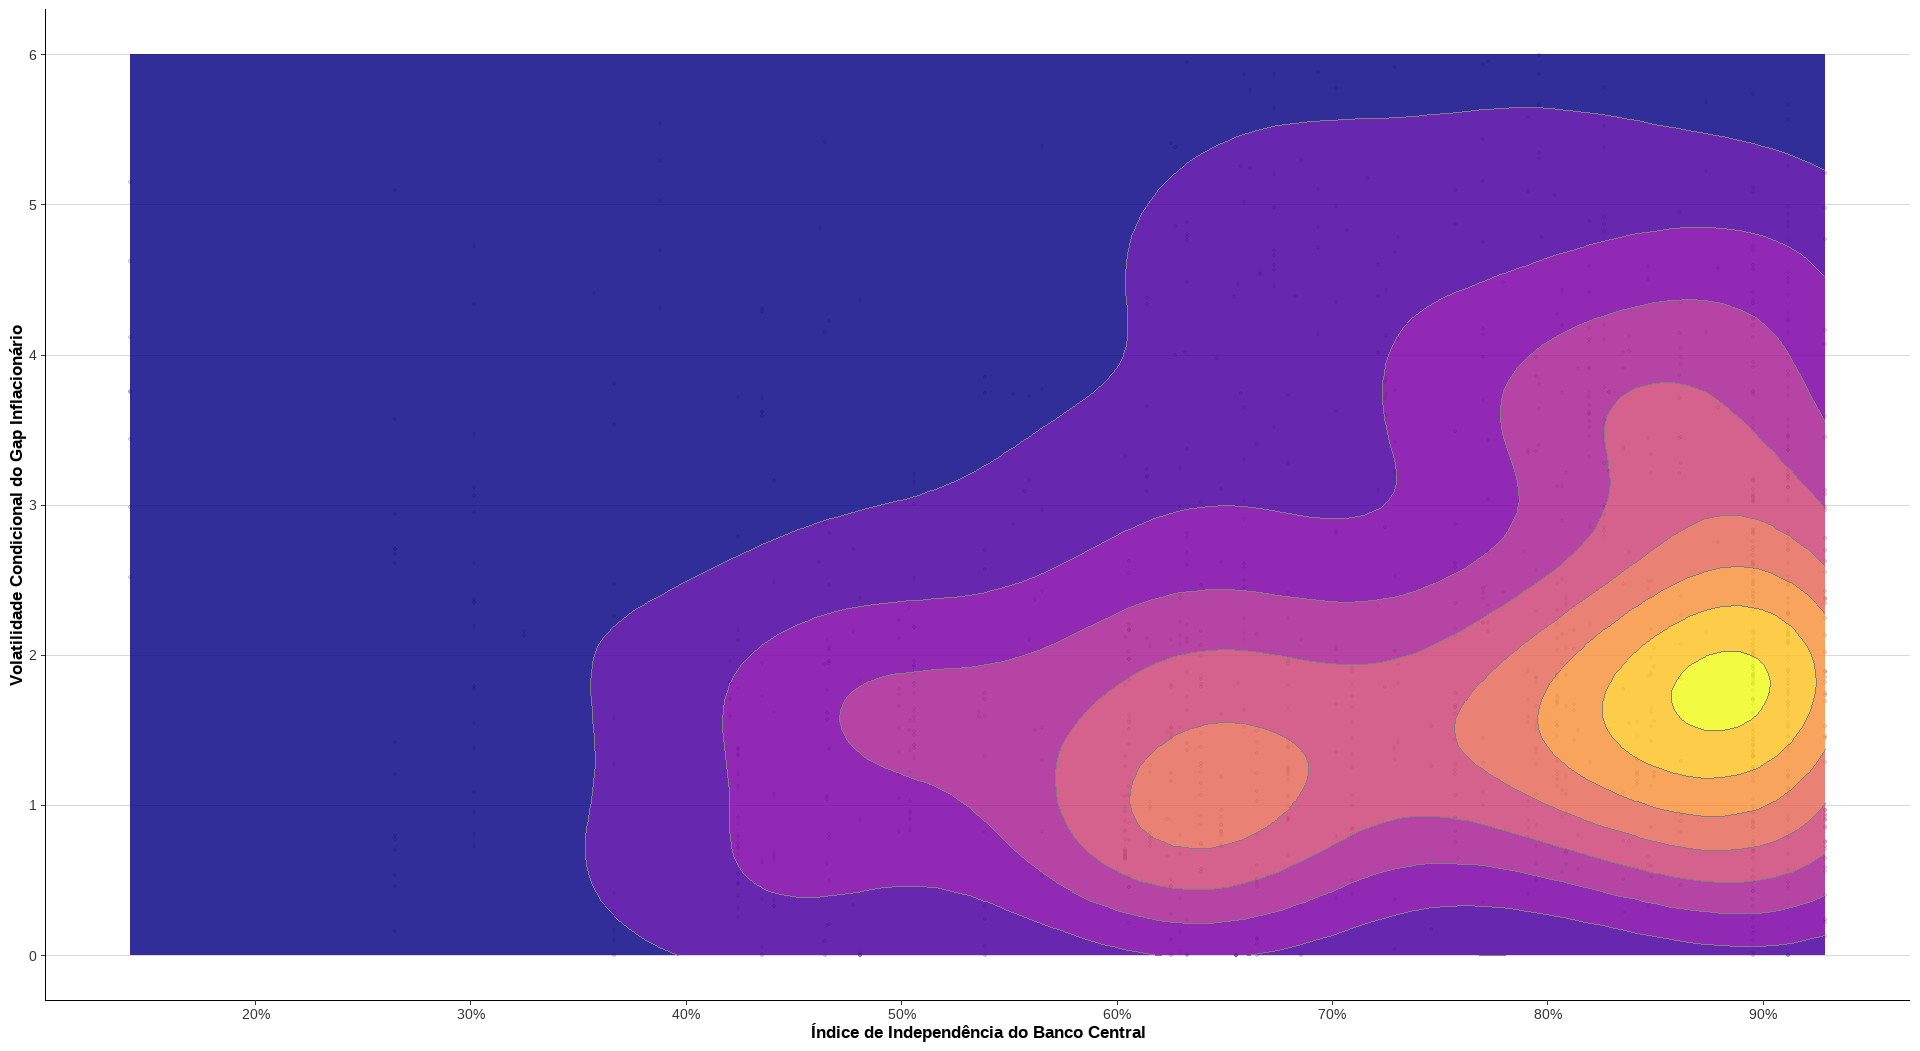
\includegraphics[width=.85\linewidth]{Imagens/paperi11.png}
    \label{fig:egarch}

    \footnotesize{Fonte: Elaborado pelos autores | WDI + FMI + CBIE}
\end{figure}

O mapa de densidade mostra concentração de baixa volatilidade do \textit{gap} em níveis de CBI acima de 60\%.  
Para valores abaixo de 50\%, a distribuição é mais dispersa, alcançando volatilidades superiores a 4p.p.  
A evidência corrobora a ideia de que a independência opera também sobre a segunda‑ordem dos choques — menor variância de erros de inflação.

\begin{figure}[H]
    \centering
    \caption{Inflação e hiato do produto por regime de independência}
    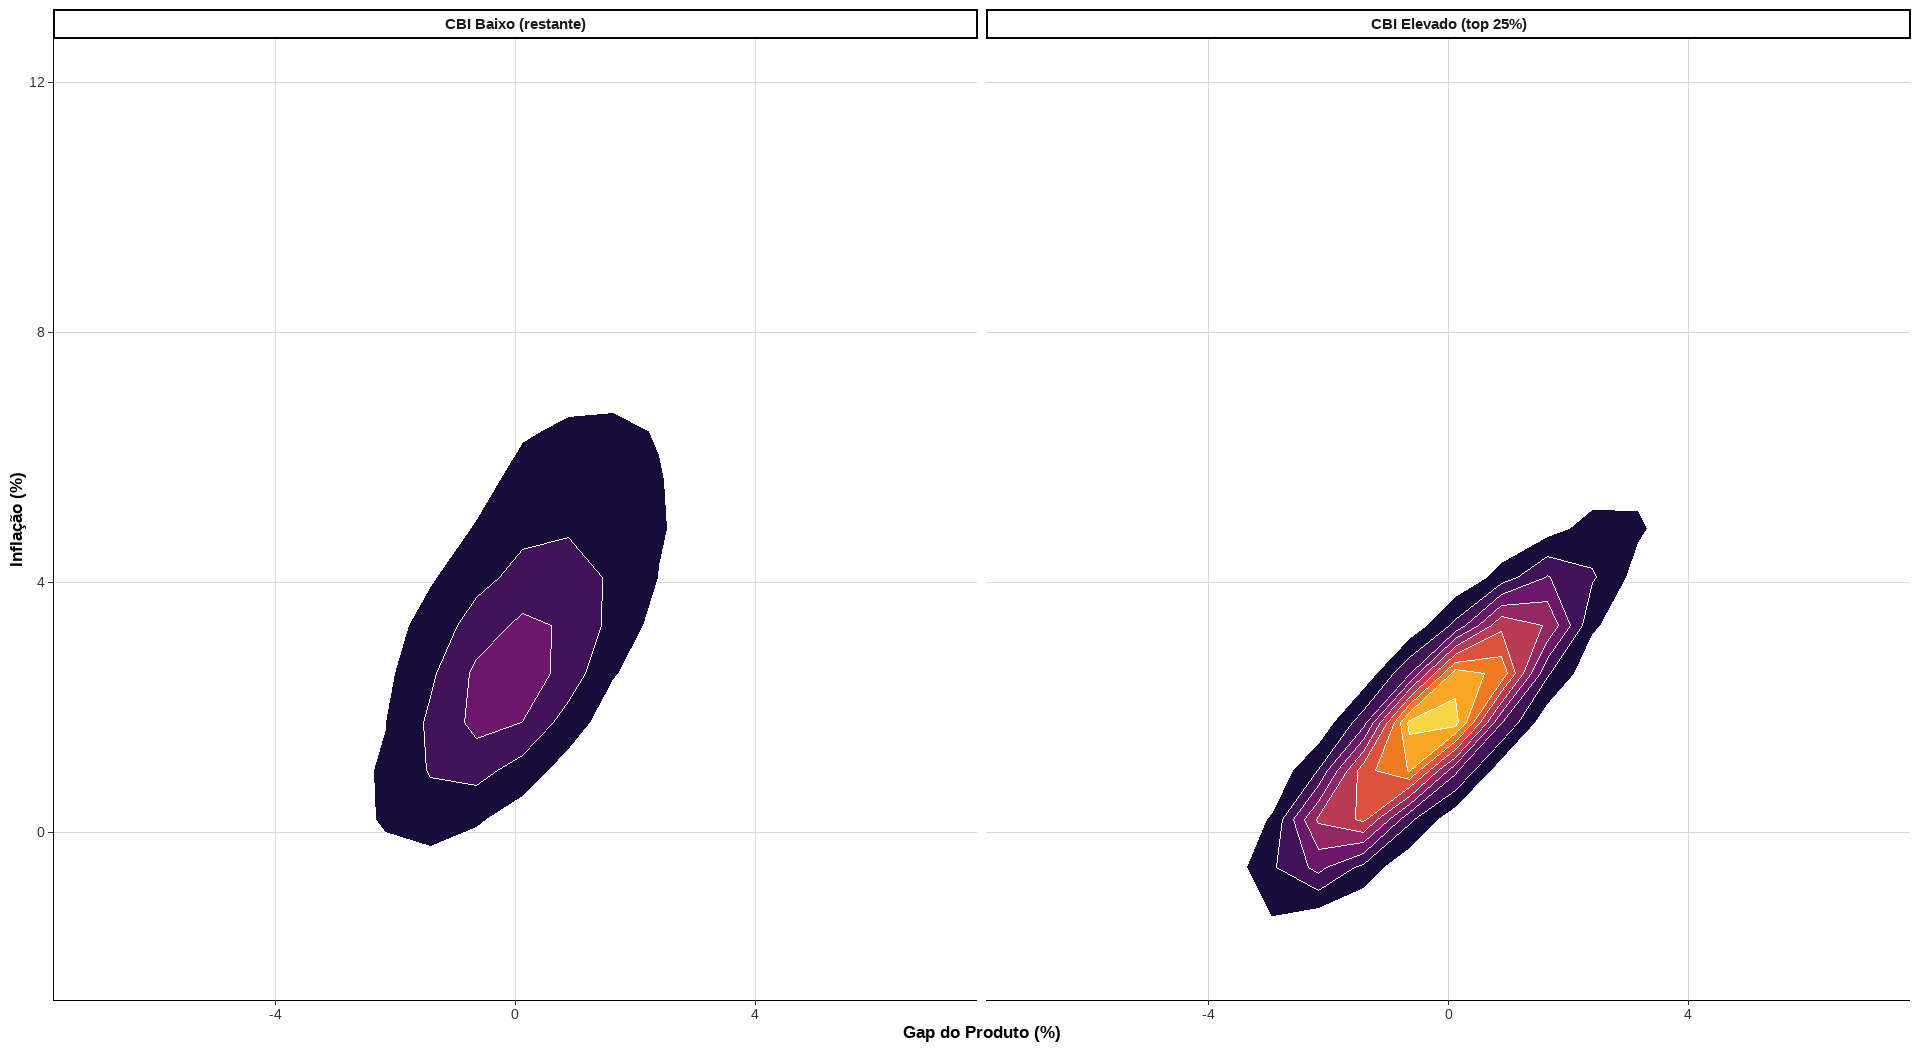
\includegraphics[width=.85\linewidth]{Imagens/paperi12.png}
    \label{fig:philips_cbi}

    \footnotesize{Fonte: Elaborado pelos autores | WDI + FMI + CBIE}
\end{figure}

O \textit{cluster} de alta independência (direita) é mais compacto e próximo da origem, apontando menores médias de inflação e hiato.  
O declive dos contornos indica sensibilidade menor da inflação ao ciclo quando o CBI é elevado, consistente com expectativas mais firmemente ancoradas.  
Já o regime de baixa independência exibe dispersão maior, sugerindo trade‑off mais instável entre atividade e preços.


\begin{figure}[H]
    \centering
    \caption{Reformas no arcabouço legal e queda subsequente da inflação}
    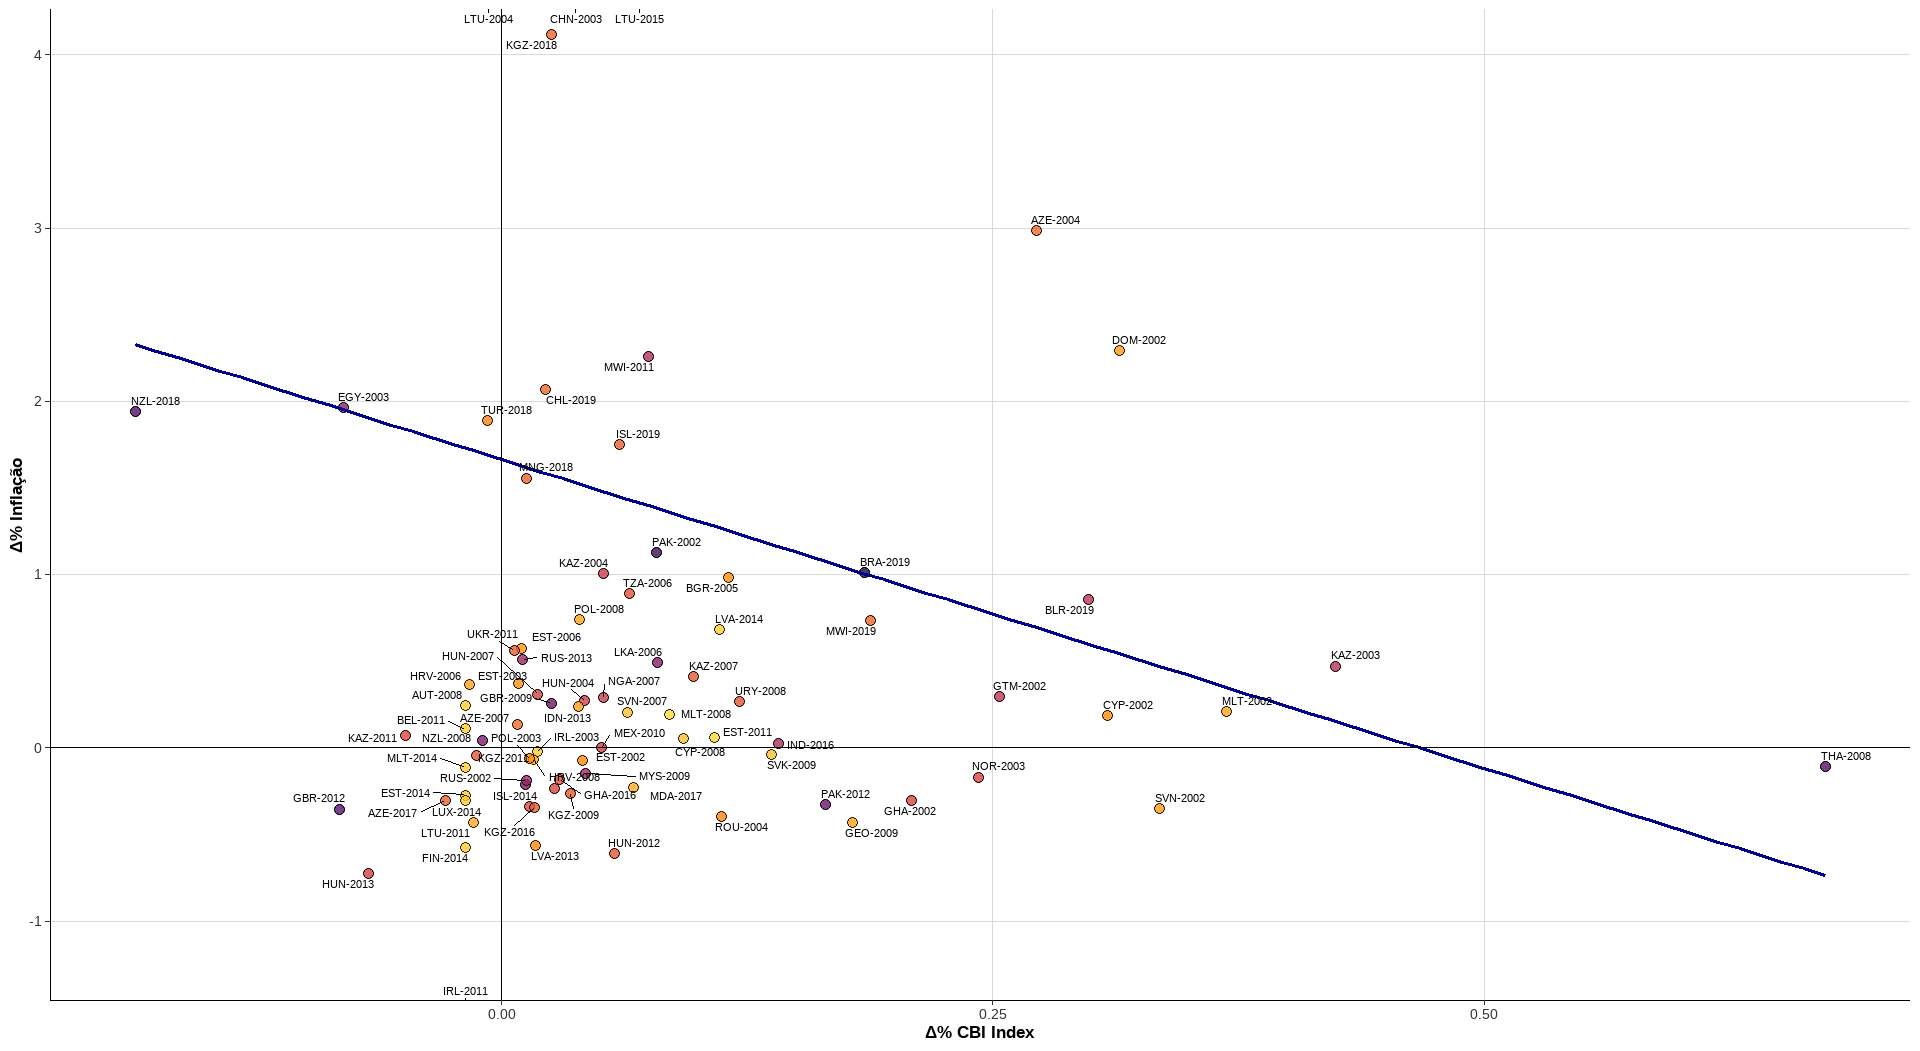
\includegraphics[width=.85\linewidth]{Imagens/paperi13.png}
    \label{fig:reforms}

    \footnotesize{Fonte: Elaborado pelos autores | WDI + FMI + CBIE}
\end{figure}

A regressão visual revela inclinação negativa: aumentos percentuais no CBI (\(\Delta\%\)) associam‑se, em média, a reduções de inflação no horizonte subsequente.  
Episódios de reforma profundos (\(\Delta\)CBI{>}0,25) concentram‑se nos quadrantes inferior direito (grande alta de CBI, forte queda de inflação), reforçando a narrativa de que mudanças institucionais robustas elevam a potência anti‑inflacionária da política monetária.


\section*{\textbf{Resultados e Discussão}}
\addcontentsline{toc}{section}{\textbf{Resultados e Discussão}}

\subsection*{\textbf{Modelo e Método de Estimação}}
\addcontentsline{toc}{subsection}{\textbf{Modelo e Método de Estimação}}

% Adicione no preâmbulo: \usepackage{amsmath}

Para testar nossa hipótese central, estimamos o seguinte modelo dinâmico:

\begin{equation}\label{eq:gmm_gap_order}
\begin{aligned}
\text{Gap inflacionário}_{it} &= \alpha_{1}(\text{Independência do BC}_{it} \times \text{Juros Real}_{it}) \\
&\quad + \alpha_{2}\text{Gap inflacionário}_{i,t-1} \\
&\quad + \alpha_{3}\text{Hiato do Produto}_{i,t-1} \\
&\quad + \alpha_{4}\text{Expectativa de inflação}_{it} \\
&\quad + \alpha_{5}\text{Independência do BC}_{it} \\
&\quad + \alpha_{6}\text{Juros Real}_{it} + \varepsilon_{it}
\end{aligned}
\end{equation}

\noindent onde $\text{Independência do BC}_{it}$ representa o Índice de Independência do Banco Central para o país $i$ no período $t$.

\textbf{Estratégia de Identificação: System-GMM}

A escolha do estimador System-GMM \cite{CameronTrivedi2005} se justifica por três características estruturais dos nossos dados:

\textbf{Persistência dinâmica}: O gap inflacionário apresenta alta persistência temporal. Em painéis com dimensão temporal limitada (\emph{small T}), a inclusão de defasagens da variável dependente em modelos de efeitos fixos gera o conhecido viés de Nickell, que pode distorcer severamente os coeficientes estimados.

\textbf{Endogeneidade contemporânea}: A taxa de juros real responde endogenamente às expectativas inflacionárias correntes, criando simultaneidade que viola a hipótese de exogeneidade estrita. O System-GMM utiliza defasagens internas como instrumentos, quebrando essa simultaneidade sem necessidade de instrumentos externos questionáveis.

\textbf{Heterogeneidade não observada}: O estimador controla simultaneamente para efeitos fixos de país ($\mu_i$) e choques temporais comuns ($\lambda_t$), removendo fontes de viés por variáveis omitidas tanto na dimensão cross-section quanto temporal.

Utilizamos defasagens de ordem superior (t-2, t-3, t-4) como instrumentos internos para as seguintes variáveis endógenas:

\begin{itemize}
    \item \textbf{Gap inflacionário}: Defasado em t-1 (persistência)
    \item \textbf{Taxa real de juros}: Contemporânea e defasada (simultaneidade)  
    \item \textbf{Expectativa de inflação}: Contemporânea (formação adaptativa)
    \item \textbf{Hiato do produto}: Defasado em t-1 (política anticíclica)
\end{itemize}

\textbf{Condições de Identificação}

O System-GMM requer o atendimento das seguintes condições:

\begin{enumerate}
    \item \textbf{Exogeneidade condicional}: $\mathbb{E}[\varepsilon_{it}|\mu_i,\lambda_t] = 0$
    \item \textbf{Validade dos momentos}: $\mathbb{E}[Z_{it}'\varepsilon_{it}] = 0$, testada via estatística de Hansen/Sargan
    \item \textbf{Ausência de correlação serial de segunda ordem}: $\mathbb{E}[\varepsilon_{it}\varepsilon_{i,t-2}] = 0$
    \item \textbf{Exogeneidade sequencial dos instrumentos}: Defasagens $t-s$ ($s \geq 2$) são ortogonais aos erros contemporâneos
\end{enumerate}

\textbf{Conjunto de Instrumentos}

Nossa estratégia instrumental utiliza as seguintes defasagens como instrumentos internos:

\begin{itemize}
    \item \texttt{Gap inflacionário}: $t-2, t-3$
    \item \texttt{Taxa real de juros}: $t-1, t-2$  
    \item \texttt{Expectativa de inflação}: $t-2, t-3$
    \item \texttt{Hiato do produto}: $t-2, t-3$
    \item \texttt{Índice de independência}: $t-1, t-2$ (tratado como pré-determinado)
\end{itemize}

\textbf{Vantagens do System-GMM}

O System-GMM apresenta vantagens comparativas significativas sobre métodos alternativos:

\textbf{Versus efeitos fixos (within)}: Não remove o viés de Nickell nem corrige simultaneidade entre taxa de juros e expectativas inflacionárias.

\textbf{Versus diferenças-em-diferenças}: Requer identificação clara de tratamento e não lida adequadamente com endogeneidade contemporânea múltipla, limitando sua aplicação em contextos macroeconômicos complexos.

\textbf{Versus IV externos}: Instrumentos monetários externos são escassos e frequentemente violam a condição de exclusão em modelos macroeconômicos, comprometendo a validade das estimativas.

\textbf{Versus GMM em diferenças}: O System-GMM combina condições de momentos em diferenças e níveis, aumentando eficiência e permitindo identificação de efeitos de variáveis invariantes no tempo, como a independência do Banco Central.

\textbf{Testes Diagnósticos}

A validade da especificação será avaliada mediante:

\begin{itemize}
    \item \textbf{Teste de Hansen/Sargan}: $H_0$: instrumentos válidos (sobre-identificação)
    \item \textbf{Teste AR(2)}: $H_0$: ausência de correlação serial de segunda ordem
    \item \textbf{Teste de diferença Hansen}: Validade de subconjuntos de instrumentos
    \item \textbf{Número de instrumentos}: Mantido abaixo do número de países para evitar sobre-ajuste
\end{itemize}

O desenho resultante é parcimonioso, evita proliferação de instrumentos e fornece base consistente para avaliar o impacto da independência do banco central sobre a eficácia da política monetária.

\subsection*{\textbf{Resultados}}
\addcontentsline{toc}{subsection}{\textbf{Resultados}}


\begin{table}[H]
    \centering
    \caption{Estimativas GMM — Índice de Independência do BC}
    \label{tab:gmm_estimates}
    \begin{tabular}{lr} 
        \toprule
        \textbf{Parâmetro} & \textbf{Resultado} \\
        \midrule
        $\alpha_1$ (Independência do BC $\times$ Taxa Real de Juros) & \makecell[r]{0.6892** \\ (0.2602)} \\
        $\alpha_2$ (Gap de Inflação Defasado) & \makecell[r]{0.2105** \\ (0.0723)} \\
        $\alpha_3$ (Hiato do Produto Defasado) & \makecell[r]{0.1824** \\ (0.0564)} \\
        $\alpha_4$ (Expectativa de Inflação) & \makecell[r]{0.6920*** \\ (0.0497)} \\
        $\alpha_5$ (Índice de Independência do BC) & \makecell[r]{-2.5699*** \\ (0.2623)} \\
        $\alpha_6$ (Taxa Real de Juros) & \makecell[r]{-0.6298** \\ (0.2200)} \\
        \midrule
        \multicolumn{2}{l}{Países (n): 78} \\
        \multicolumn{2}{l}{Observações (N): 1869} \\
        \multicolumn{2}{l}{Significância: *** p<0.001; ** p<0.01; * p<0.05} \\
        \multicolumn{2}{l}{Wald: $\chi^2(6) = 51803.945$ (p = $<$2e-16)} \\
        \multicolumn{2}{l}{AR(1): z = -2.306 (p = 0.021)} \\
        \multicolumn{2}{l}{AR(2): z = 1.381 (p = 0.167)} \\
        \bottomrule
    \end{tabular}
    
    \footnotesize{Fonte: Próprios autores | Saída GMM-System}.
\end{table}

O coeficiente da interação entre o índice de independência do BC e a taxa real de juros ($\alpha_1$ = 0,6892) é positivo e estatisticamente significativo a 1\%, sugerindo que quanto maior a independência do BC, maior é a potência da política monetária, ou seja, os efeitos da taxa de juros sobre a inflação se tornam mais pronunciados. Isso indica que a autonomia institucional do BC amplifica a efetividade da política monetária.

O coeficiente do gap de inflação defasado ($\alpha_2$ = 0,2105) confirma a existência de inércia inflacionária, com valores passados de inflação influenciando a inflação atual. Da mesma forma, o hiato do produto defasado ($\alpha_3$ = 0,1824) apresenta sinal positivo e significativo, indicando que uma economia operando acima do seu potencial tende a pressionar os preços para cima.

A expectativa de inflação ($\alpha_4$ = 0,6920) tem um efeito elevado e altamente significativo, o que reforça o papel central das expectativas no processo inflacionário, conforme previsto pela teoria Neo-Keynesiana.

O índice de independência do Banco Central, considerado de forma isolada ($\alpha_5$ = -2,6999), mostra um efeito negativo e significativo sobre a inflação, o que evidencia que maiores níveis de autonomia institucional estão associados a menores taxas inflacionárias, mesmo sem considerar a interação com os juros.

Por fim, a taxa real de juros isolada ($\alpha_6$ = -0,6298) também reduz a inflação, mas seu efeito é menos intenso do que quando combinado com a independência do BC, reforçando a ideia de que a autonomia da autoridade monetária potencializa os canais de transmissão da política monetária.

\subsubsection*{\textbf{Robustez}}
\addcontentsline{toc}{subsubsection}{\textbf{Robustez}}

\begin{table}[H]
    \centering
    \caption{Estimativas GMM — Índice de Independência do BC (Fiscal)}
    \label{tab:gmm_fiscal_estimates}
    \begin{tabular}{lr} 
        \toprule
        \textbf{Parâmetro} & \textbf{Resultado} \\
        \midrule
        $\alpha_1$ (Independência do BC $\times$ Taxa Real de Juros) & \makecell[r]{0.7935* \\ (0.3408)} \\
        $\alpha_2$ (Gap de Inflação Defasado) & \makecell[r]{0.2201** \\ (0.0678)} \\
        $\alpha_3$ (Hiato do Produto Defasado) & \makecell[r]{0.2441*** \\ (0.0625)} \\
        $\alpha_4$ (Expectativa de Inflação) & \makecell[r]{0.6701*** \\ (0.0563)} \\
        $\alpha_5$ (Índice de Independência do BC) & \makecell[r]{-2.4294*** \\ (0.2848)} \\
        $\alpha_6$ (Taxa Real de Juros) & \makecell[r]{-0.7130* \\ (0.2828)} \\
        $\alpha_7$ (Impulso Fiscal) & \makecell[r]{-0.0945** \\ (0.0333)} \\
        \midrule
        \multicolumn{2}{l}{Países (n): 78} \\
        \multicolumn{2}{l}{Observações (N): 1869} \\
        \multicolumn{2}{l}{Significância: *** p<0.001; ** p<0.01; * p<0.05} \\
        \multicolumn{2}{l}{Wald: $\chi^2(7) = 18860.828$ (p = $<$2e-16)} \\
        \multicolumn{2}{l}{AR(1): z = -4.19 (p = 0)} \\
        \multicolumn{2}{l}{AR(2): z = 12.439 (p = 0)} \\
        \bottomrule
    \end{tabular}

    \footnotesize{Fonte: Próprios autores | Saída GMM-System}.
\end{table}

A Tabela 4 apresenta os resultados do modelo que inclui, além das variáveis tradicionais de política monetária, o impacto do impulso fiscal, com o objetivo de avaliar como a independência do Banco Central (BC), agora sob uma ótica fiscal, influencia a eficácia da política monetária no controle da inflação.

O principal destaque está na interação entre a independência do BC e a taxa real de juros ($\alpha_1$ = 0,7935), que permanece positiva e significativa ao nível de 5\%. Isso reforça a conclusão de que a autonomia do BC aumenta a potência da política monetária, tornando os juros reais mais eficazes no combate à inflação. Esse efeito é ligeiramente mais forte do que o observado na Tabela 3, sugerindo que o contexto fiscal também potencializa essa relação.

Outros coeficientes mantêm padrões semelhantes. O gap de inflação defasado ($\alpha_2$ = 0,2201) e o hiato do produto defasado ($\alpha_3$ = 0,2414) continuam a apresentar efeitos positivos e estatisticamente significativos, indicando que tanto a inflação passada quanto o grau de atividade econômica afetam a inflação corrente. A expectativa de inflação ($\alpha_4$ = 0,6925) novamente se mostra altamente relevante, apontando seu papel central na dinâmica inflacionária.

O coeficiente da independência do Banco Central ($\alpha_5$ = -2,4294) segue sendo negativo e estatisticamente significativo, confirmando que um maior grau de autonomia institucional está associado a menores níveis de inflação. A taxa real de juros isoladamente ($\alpha_6$ = -0,7130) também reduz a inflação, e de forma mais intensa do que no modelo anterior, o que pode refletir uma maior sensibilidade da inflação às condições monetárias em cenários com mais variabilidade fiscal.

Por fim, o impulso fiscal ($\alpha_7$ = -0,0945) apresenta sinal negativo e estatisticamente significativo. Isso sugere que políticas fiscais expansionistas (impulsos fiscais positivos) contribuem para a redução da inflação.

\begin{table}[H]
    \centering
    \caption{Estimativas GMM — Independência do BC (Política Monetária)}
    \label{tab:gmm_monetary_estimates}
    \begin{tabular}{lr} 
        \toprule
        \textbf{Parâmetro} & \textbf{Resultado} \\
        \midrule
        $\alpha_1$ (Independência do BC (PM) $\times$ Taxa Real de Juros) & \makecell[r]{1.1196* \\ (0.4487)} \\
        $\alpha_2$ (Gap de Inflação Defasado) & \makecell[r]{0.2205*** \\ (0.0661)} \\
        $\alpha_3$ (Hiato do Produto Defasado) & \makecell[r]{0.2216*** \\ (0.0588)} \\
        $\alpha_4$ (Expectativa de Inflação) & \makecell[r]{0.6815*** \\ (0.0539)} \\
        $\alpha_5$ (Índice de Independência do BC - Política Monetária) & \makecell[r]{-2.9034*** \\ (0.3111)} \\
        $\alpha_6$ (Taxa Real de Juros) & \makecell[r]{-0.9218** \\ (0.3531)} \\
        $\alpha_7$ (Impulso Fiscal) & \makecell[r]{-0.0713* \\ (0.0348)} \\
        \midrule
        \multicolumn{2}{l}{Países (n): 78} \\
        \multicolumn{2}{l}{Observações (N): 1869} \\
        \multicolumn{2}{l}{Significância: *** p<0.001; ** p<0.01; * p<0.05} \\
        \multicolumn{2}{l}{Wald: $\chi^2(7) = 72315.01$ (p = $<$2e-16)} \\
        \multicolumn{2}{l}{AR(1): z = -2.896 (p = 0.004)} \\
        \multicolumn{2}{l}{AR(2): z = 1.964 (p = 0.049)} \\
        \bottomrule
    \end{tabular}

    \footnotesize{Fonte: Próprios autores | Saída GMM-System}.
\end{table}

A Tabela 5 mostra os resultados do modelo, que busca avaliar como a independência do Banco Central na condução da política monetária.

O coeficiente $\alpha_1$, que representa a interação entre a independência do BC na definição da taxa de juros e a taxa real de juros, tem valor positivo (1.1196) e é estatisticamente significativo ao nível de 5\%. Isso indica que, quando o Banco Central possui autonomia institucional para decidir a taxa de juros, o efeito da política monetária sobre a inflação é ampliado. Em outras palavras, a independência fortalece a potência dos juros como instrumento de combate à inflação.

O coeficiente $\alpha_2$, que mede o efeito do gap de inflação defasado, é positivo (0.2205) e altamente significativo. Isso confirma a existência de inércia inflacionária: a inflação passada exerce influência direta sobre a inflação atual. Já o coeficiente $\alpha_3$, referente ao hiato do produto defasado, também é positivo (0.2216) e altamente significativo, indicando que uma economia aquecida, operando acima de seu produto potencial, tende a gerar maior pressão inflacionária.

A expectativa de inflação, $\alpha_4$, apresenta uma estimativa de 0.6815 e é altamente significativa. Esse resultado reforça o papel crucial das expectativas na determinação da inflação corrente, coerente com a literatura Neo-Keynesiana, que destaca a importância da credibilidade do regime monetário na ancoragem das expectativas.

O coeficiente $\alpha_5$, que representa o efeito direto da independência do Banco Central sobre a inflação, tem valor negativo (-2.9034) e é altamente significativo. Isso sugere que, independentemente da taxa de juros, maior autonomia da autoridade monetária está associada a menores taxas de inflação. Esse é um dos principais achados do modelo, ao evidenciar que a estrutura institucional afeta diretamente o desempenho inflacionário.

A taxa real de juros isoladamente, representada por $\alpha_6$, possui coeficiente negativo (-0.9218) e é significativa ao nível de 1\%. Isso indica que, mesmo fora da interação com a independência, o aumento dos juros reais tem um efeito direto de contenção inflacionária, conforme previsto pela teoria econômica convencional.

Por fim, o impulso fiscal, representado por $\alpha_7$, tem coeficiente negativo (-0.0713) e é significativo ao nível de 5\%. Isso mostra que políticas fiscais mais expansionistas (como a aumento de gastos ou redução de arrecadação) também contribuem para a desaceleração da inflação.

\begin{table}[H]
    \centering
    \caption{Estimativas GMM — Independência do BC (Política Monetária Q1)}
    \label{tab:gmm_monetary_q1_estimates}
    \begin{tabular}{lr} 
        \toprule
        \textbf{Parâmetro} & \textbf{Resultado} \\
        \midrule
        $\alpha_1$ (Independência do BC (PM Q1) $\times$ Taxa Real de Juros) & \makecell[r]{1.2564 \\ (0.7073)} \\
        $\alpha_2$ (Gap de Inflação Defasado) & \makecell[r]{0.2282*** \\ (0.0675)} \\
        $\alpha_3$ (Hiato do Produto Defasado) & \makecell[r]{0.2346*** \\ (0.0589)} \\
        $\alpha_4$ (Expectativa de Inflação) & \makecell[r]{0.6754*** \\ (0.0506)} \\
        $\alpha_5$ (Índice de Independência do BC - Política Monetária Q1) & \makecell[r]{-2.0673*** \\ (0.2215)} \\
        $\alpha_6$ (Taxa Real de Juros) & \makecell[r]{-1.3040 \\ (0.7016)} \\
        $\alpha_7$ (Impulso Fiscal) & \makecell[r]{-0.0933** \\ (0.0314)} \\
        \midrule
        \multicolumn{2}{l}{Países (n): 78} \\
        \multicolumn{2}{l}{Observações (N): 1869} \\
        \multicolumn{2}{l}{Significância: *** p<0.001; ** p<0.01; * p<0.05} \\
        \multicolumn{2}{l}{Wald: $\chi^2(7) = 20374.249$ (p = $<$2e-16)} \\
        \multicolumn{2}{l}{AR(1): z = -2.525 (p = 0.012)} \\
        \multicolumn{2}{l}{AR(2): z = 1.842 (p = 0.065)} \\
        \bottomrule
    \end{tabular}

    \footnotesize{Fonte: Próprios autores | Saída GMM-System}.
\end{table}
A Tabela 6 apresenta os resultados do modelo que investiga os efeitos da independência do Banco Central (BC), com foco específico no componente que mede a autonomia do BC em relação a decisão da ferramenta de política monetária (taxa de juros).

O coeficiente da interação entre esse índice (Q1) e a taxa real de juros ($\alpha_1$ = 1,2564), embora não significativo estatisticamente, é positivo e numericamente expressivo. Isso sugere que, em países onde o BC tem autoridade formal para definir a taxa de juros, a política monetária tende a ser mais potente — ou seja, os juros reais exercem maior influência sobre a inflação. A ausência de significância estatística pode estar associada a heterogeneidade institucional ou a ruídos nos dados, mas o sinal do coeficiente corrobora a hipótese teórica.

Os coeficientes das variáveis de controle reforçam os achados consistentes nas tabelas anteriores: o gap de inflação defasado ($\alpha_2$ = 0,2282) e o hiato do produto ($\alpha_3$ = 0,2346) indicam que tanto a inércia inflacionária quanto o nível de atividade econômica têm efeitos positivos sobre a inflação. A expectativa de inflação ($\alpha_4$ = 0,6754), altamente significativa, reafirma seu papel central no processo de formação de preços.

O componente específico do índice de independência relacionado à decisão sobre juros (Q1), isoladamente ($\alpha_5$ = -2,0673), apresenta efeito negativo e altamente significativo, indicando que países cujo BC tem autonomia institucional para definir a taxa de juros tendem a apresentar menor inflação. Trata-se de uma evidência robusta do papel direto da independência monetária na estabilidade de preços.

A taxa real de juros ($\alpha_6$ = -1,0436) também apresenta coeficiente negativo, mas sem significância estatística neste modelo, sugerindo que sua eficácia depende diretamente da presença de autonomia decisória do BC, ou seja, sem independência, os juros sozinhos perdem força como instrumento anti-inflacionário.

O impulso fiscal ($\alpha_7$ = -0,0933) mostra-se estatisticamente significativo e negativo, reforçando o papel complementar da política fiscal: uma política fiscal menos restritiva contribui para conter a inflação.

\subsection*{\textbf{Uma Análise \textit{ceteris paribus}}}
\addcontentsline{toc}{subsection}{\textbf{Uma Análise \textit{ceteris paribus}}}

\begin{table}[htbp]
    \centering
    \caption{Comparativo de Parâmetros por Caso e País} % Título da tabela
    \label{tab:comparative_cases}
    % Usando adjustbox para garantir que a tabela caiba na largura da página, se ficar muito larga
    % \begin{adjustbox}{max width=\textwidth}
    \begin{tabular}{l rr rr rr} % 1 coluna para Parâmetro (l), e 2 (rr) para cada um dos 3 casos
        \toprule
        % Cabeçalho principal para os Casos
        \multicolumn{1}{l}{\textbf{}} & \multicolumn{2}{c}{\textbf{Caso 1}} & \multicolumn{2}{c}{\textbf{Caso 2}} & \multicolumn{2}{c}{\textbf{Caso 3}} \\
        % Linhas menores para País 1 e País 2 dentro de cada Caso
        \cmidrule(lr){2-3} \cmidrule(lr){4-5} \cmidrule(lr){6-7}
        \textbf{Parâmetro} & \textbf{País 1} & \textbf{País 2} & \textbf{País 1} & \textbf{País 2} & \textbf{País 1} & \textbf{País 2} \\
        \midrule
        Gap de Inflação Defasado & 0,8 & 0,8 & 0,8 & 0,8 & 0,8 & 0,8 \\
        Hiato do Produto Defasado(\%) & 1,2 & 1,2 & 1,2 & 1,2 & 1,2 & 1,2 \\
        Expectativa de Inflação(\%) & 4,5 & 4,5 & 4,5 & 4,5 & 4,5 & 4,5 \\
        Índice de Independência do BC & 0,6 & 0,8 & 0,6 & 0,8 & 0,6 & 0,8 \\
        Taxa Real de Juros(\%) & 0,6 & 0,6 & 3,7 & 3,7 & 4 & 4 \\
        \midrule
        Estimava (p.p) & 1,83 & 1,40 & 1,16 & 1,16 & 1,09 & 1,13 \\
        \bottomrule
    \end{tabular}
    % \end{adjustbox}

        \footnotesize{Fonte: Próprios autores}.
\end{table}

A análise dos resultados empíricos pode ser ilustrada por meio de três cenários hipotéticos. No Caso 1, observa-se que o País 1, com um índice de Independência de 0,60, apresentaria um GAP esperado de 1,83 pontos percentuais, situando-se acima da meta de inflação. Por outro lado, o País 2, com um índice de Independência de 0,80, apresentaria um GAP esperado ligeiramente menor, de 1,40 pontos percentuais, mas ainda assim acima da meta.

No Caso 2, os resultados apresentam dinâmica distinta. O País 1, mantendo um mesmo grau de Independência (0,60), teria um GAP esperado de 1,16 pontos percentuais, também acima da meta. Curiosamente, o País 2, com Independência de 0,80, também teira um GAP esperado de 1,16 pontos percentuais, igualmente acima da meta, sugerindo ausência de ganho adicional em termos de convergência à meta neste cenário.

Por fim, no Caso 3, ao observar o País 1, com Independência de 0,60, geraria a um GAP esperado de 1,09 pontos percentuais, ainda acima da meta. E o País 2, com seu índice de Independência de 0,80, teria um GAP esperado de 1,13 pontos percentuais, ambos superando a meta inflacionária.


\section*{\textbf{Conclusão}}
\addcontentsline{toc}{section}{\textbf{Conclusão}}

A análise do modelo converge para uma conclusão crucial: a maior independência formal do Banco Central (BC) não se traduz, NECESSARIAMENTE, em um aumento da potência ou eficácia de sua Política Monetária. Este achado sugere que a autonomia institucional, embora importante, não é o único ou o principal determinante da capacidade de intervenção e impacto do BC na economia.

Contudo, a interpretação desses resultados deve ser realizada com a devida consideração às limitações inerentes ao estudo. Em termos de dados, enfrentamos desafios significativos, como a impossibilidade de obter uma série histórica de longo prazo para a expectativa de inflação, o que pode restringir a abrangência temporal da análise. Além disso, a escassez de dados consistentes sobre a dívida pública para um número amplo de países ao longo dos anos limita a capacidade de generalização dos achados. O caráter desbalanceado do painel de dados, por sua vez, introduz uma complexidade que exige cautela na interpretação dos resultados, podendo gerar vieses ou incertezas.

Outra limitação relevante reside na baixa variação temporal do Índice de Independência do Banco Central (CBI), o que pode dificultar a identificação de um efeito causal robusto nas análises de regressão. A validade dos índices de independência utilizados, como os de Acemoglu, pode ser questionada devido a possíveis desatualizações. Adicionalmente, o estudo reconhece a dificuldade intrínseca em mensurar e identificar a verdadeira potência da política monetária e em garantir a exogeneidade do índice CBI, o que é crucial para inferências causais. Por fim, é fundamental notar que o modelo não controlou para um possível "efeito gangorra", que poderia distorcer as relações observadas, e que o índice CBI avalia a independência apenas do ponto de vista legal ('de jure'), e não a independência efetiva na prática ('de facto'), o que pode apresentar uma dicotomia importante para a realidade operacional dos Bancos Centrais. Essas ressalvas são essenciais para uma compreensão completa das implicações do modelo.


% Conteúdo da Conclusão aqui...


\newpage
\printbibliography
\addcontentsline{toc}{section}{\textbf{Bibliografia}}

\newpage
\section*{Reprodução}
\addcontentsline{toc}{section}{\textbf{Reprodução}}


Este trabalho foi desenvolvido seguindo princípios de ciência aberta e reprodutibilidade. Todo o código, dados e documentação necessários para replicar integralmente os resultados estão disponíveis publicamente no repositório GitHub. A estrutura do repositório foi organizada de forma a garantir reprodutibilidade total da análise, desde a coleta de dados até a geração dos resultados finais.

\subsection*{Estrutura de Arquivos}

\subsubsection*{Dados Primários}

A pasta \texttt{Data} contém 5 arquivos \texttt{.xlsx} fundamentais:

\begin{enumerate}
    \item \textbf{CBIDta.xlsx}: Base de dados sobre independência dos bancos centrais (CBIE) desenvolvida por Romelli (2022, 2024), cobrindo 155 países entre 1923 e 2023. Este arquivo constitui a fonte principal para os índices de independência utilizados nas estimações.
    
    \item \textbf{InflationForecast(FMI).xlsx}: Projeções de inflação extraídas das bases de dados do Fundo Monetário Internacional, essenciais para a construção da variável de expectativas inflacionárias utilizada no modelo Novo-Keynesiano.
    
    \item \textbf{rate\_macrobond.xlsx}: Série histórica de taxas de juros nominais dos bancos centrais, coletadas via plataforma Macrobond, utilizadas para o cálculo das taxas reais de juros.
    
    \item \textbf{target(eikon).xlsx}: Metas de inflação oficiais divulgadas pelos bancos centrais, obtidas via sistema Eikon (LSEG), fundamentais para o cálculo do gap inflacionário.
    
    \item \textbf{target(macrobond).xlsx}: Metas de inflação complementares obtidas via Macrobond, com foco prioritário em países da Zona do Euro, garantindo maior cobertura temporal e geográfica.
\end{enumerate}

\subsubsection*{Scripts e Documentação}

O repositório inclui os seguintes arquivos de código e documentação:

\begin{itemize}
    \item \textbf{PEE.R}: Script principal contendo todas as etapas de importação, limpeza, transformação de dados, cálculo de variáveis derivadas e estimações econométricas. O código está estruturado de forma modular, com comentários detalhados para facilitar a compreensão e replicação.
    
    \item \textbf{PEE.Rmd}: Documento R Markdown que integra código, análise e narrativa do trabalho, permitindo a geração automática de relatórios com resultados atualizados.
    
    \item \textbf{Base de Dados.md}: Script automatizado para download e organização dos dados diretamente via GitHub, garantindo acesso facilitado aos dados originais.
    
    \item \textbf{README.md}: Documentação completa do projeto, incluindo metodologia detalhada, instruções de execução, requisitos de software e orientações para replicação dos resultados.
\end{itemize}

\subsection*{Links de Acesso}

\textbf{Repositório Principal}: \\
\url{https://github.com/Hic-Tayfour/R/tree/main/College%20Works/PEE%202025.1}

\textbf{Script Markdown (HTML)}: \\
\url{https://raw.githack.com/Hic-Tayfour/HTML/refs/heads/main/PEE.html}

\subsubsection*{Acesso Direto aos Arquivos}

Para facilitar a replicação, os principais componentes estão organizados da seguinte forma:

\begin{itemize}
    \item \textbf{Código principal}: Disponível no repositório principal com estrutura modular
    \item \textbf{Resultados compilados}: Versão HTML interativa com todos os outputs
    \item \textbf{Dados processados}: Arquivos intermediários para verificação de etapas
    \item \textbf{Documentação técnica}: README detalhado com especificações do ambiente
\end{itemize}

\subsection*{Licença e Acesso}

Os dados e códigos estão disponibilizados sob licença aberta, permitindo uso acadêmico e educacional. A transparência metodológica visa contribuir para o avanço do conhecimento científico na área de economia monetária e facilitar futuras pesquisas sobre independência de bancos centrais.

\textit{Todos os links foram testados e garantem acesso direto aos materiais necessários para reprodução completa dos resultados.}

\end{document}

% ---------------------------------------------------
%  Introdução e Formulação do Problema
% ---------------------------------------------------
\section*{\textbf{Introdução e Formulação do Problema}}
\addcontentsline{toc}{section}{\textbf{Introdução e Formulação do Problema}}

A credibilidade do Banco Central (BC) é um dos pilares para a efetividade da política monetária. Conforme ressalta \cite{fischer1994}, “\emph{more independent central banks deliver better outcomes, particularly lower and more stable inflation}”.%
\footnote{FISCHER, Stanley. \textit{Central bank independence revisited}. BIS Review, n.~55, 1994. Disponível em: \url{https://www.bis.org/review/r151109c.htm}. Acesso em: 11 jun. 2025.}%

Em reflexão posterior, \cite{fischer2015} enfatiza que “\emph{instrument independence is indispensable, for without it the central bank is unable to set the stance of monetary policy most consistent with achievement of the statutory mandate}.”%
\footnote{FISCHER, Stanley. \textit{Central bank independence}. Discurso proferido no National Economists Club, Washington, D.C., 4 nov. 2015. Disponível em: \url{https://www.federalreserve.gov/newsevents/speech/fischer20151104a.htm}. Acesso em: 11 jun. 2025.}  

Essas afirmações reforçam que a autonomia institucional amplia a potência da política monetária ao ancorar expectativas e reduzir interferências de curto prazo.

Diante da relevância do tema e das experiências recentes no contexto brasileiro e internacional, este estudo adota o seguinte \textbf{tema} de investigação:

\begin{center}
\vspace{0.5em}
\textbf{\Large Independência do BC e a Potência da Política Monetária}
\vspace{0.5em}
\end{center}

% ---------------------------------------------------
%  Motivação
% ---------------------------------------------------
\section*{\textbf{Motivação}}
\addcontentsline{toc}{section}{\textbf{Motivação}}

Christine Lagarde (2025)\footnote{LAGARDE, Christine. \textit{Central bank independence in an era of volatility}. Discurso proferido em 27 jan. 2025. Frankfurt: European Central Bank, 2025. Disponível em: \url{https://www.ecb.europa.eu/press/key/date/2025/html/ecb.sp250127~16c35af0c0.en.html}. Acesso em: 06 jun. 2025.} argumenta que, em meio à atual “era de volatilidade”, a autonomia é ainda mais crucial para que os bancos centrais tomem decisões difíceis, preservem a âncora das expectativas e, assim, contenham a propagação de choques inflacionários. Embora mais de 80 \% dos BCs tenham conquistado independência operacional no fim do século XX, Lagarde observa que pressões políticas pós-2008 ameaçam esse avanço, podendo elevar a volatilidade macroeconômica caso a credibilidade das autoridades monetárias seja minada.

Athanassopoulos, Masciandaro e Romelli (2025)\footnote{ATHANASOPOULOS, Angelos; MASCIANDARO, Donato; ROMELLI, Davide. \textit{It matters even more: Central bank independence, long-run inflation, and persistence}. VoxEU, 18 fev. 2025. Disponível em: \url{https://cepr.org/voxeu/columns/it-matters-even-more-central-bank-independence-long-run-inflation-and-persistence}. Acesso em: 06 jun. 2025.} mostram, com modelos dinâmicos para 155 países, que reformas que ampliam a independência reduzem a inflação de longo prazo de forma mais acentuada do que no curto prazo e diminuem a persistência inflacionária. Os ganhos são especialmente fortes em economias em desenvolvimento, reforçando o argumento de que, onde a credibilidade ainda se constrói, a autonomia do BC é um instrumento decisivo para tornar a política monetária mais potente.

Em painel nas Reuniões de Primavera do FMI, Gita Gopinath destacou que a elevada incerteza global dificulta a calibragem da política monetária e aumenta a pressão sobre os bancos centrais. Ao citar o episódio de tensão entre Donald Trump e Jerome Powell, ela reforçou que a independência é “muito importante para a estabilidade econômica”\footnote{CNN BRASIL. \textit{Alta incerteza global dificulta política monetária e pressiona BCs, diz FMI}. 25 abr. 2025. Disponível em: \url{https://www.cnnbrasil.com.br/economia/macroeconomia/alta-incerteza-global-dificulta-politica-monetaria-e-pressiona-bcs-diz-fmi/}. Acesso em: 06 jun. 2025.}. Segundo o FMI, choques protecionistas e movimentos abruptos nos rendimentos dos Treasuries americanos ilustram como pressões externas complicam o trabalho das autoridades monetárias — motivo adicional para preservar sua autonomia decisória.

O debate sobre a independência do Banco Central é particularmente pertinente em economias emergentes como a brasileira, onde pressões políticas e choques fiscais tendem a comprometer a credibilidade das instituições.  A autonomia formal da autoridade monetária tem se destacado como instrumento para melhorar a previsibilidade da política de juros e a estabilidade macroeconômica de longo prazo.

Como argumentado por \cite{adrian2024}, o desenvolvimento de novos índices de independência permite uma análise mais refinada sobre a relação entre autonomia e eficácia na condução monetária.  A Figura~\ref{fig:comparacao_bc} apresenta uma comparação esquemática entre um Banco Central independente e outro sujeito a pressões políticas.

\end{document}

% ---------------------------------------------------
%  Motivação
% ---------------------------------------------------
\section{Motivação}

O debate sobre a independência do Banco Central é particularmente pertinente em economias emergentes como a brasileira, onde pressões políticas e choques fiscais tendem a comprometer a credibilidade das instituições.  A autonomia formal da autoridade monetária tem se destacado como instrumento para melhorar a previsibilidade da política de juros e a estabilidade macroeconômica de longo prazo.  Na mesma linha, \citeauthor{fischer2017} (\citeyear{fischer2017}) sustenta que a flexibilidade derivada da independência foi crucial para o Federal Reserve criar novos instrumentos e, assim, evitar uma recessão mais profunda nos Estados Unidos durante a crise de 2008.

Como argumentado por \cite{adrian2024}, o desenvolvimento de novos índices de independência permite uma análise mais refinada sobre a relação entre autonomia e eficácia na condução monetária.  A Figura~\ref{fig:comparacao_bc} apresenta uma comparação esquemática entre um Banco Central independente e outro sujeito a pressões políticas.

\begin{figure}[H]
    \centering
    \begin{subfigure}[b]{0.45\textwidth}
        \centering
        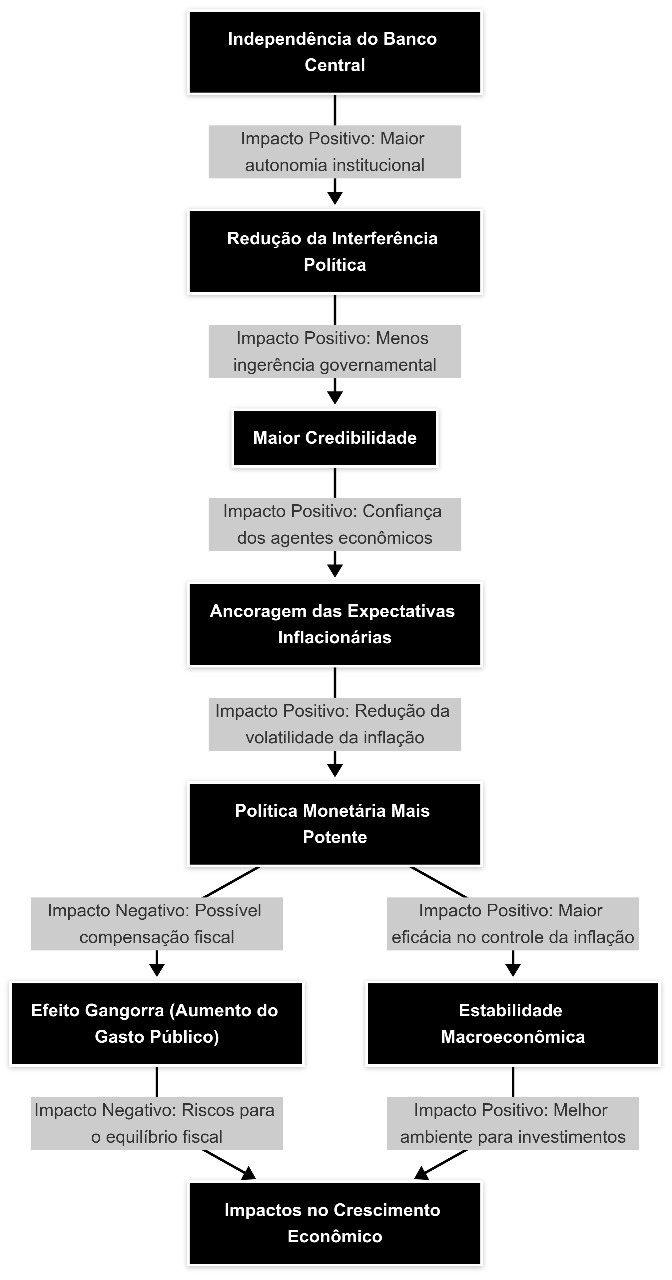
\includegraphics[width=\linewidth]{Imagens/m2i1.jpg}
        \caption{Banco Central Independente}
        \label{fig:bc_independente}
    \end{subfigure}
    \hfill
    \begin{subfigure}[b]{0.45\textwidth}
        \centering
        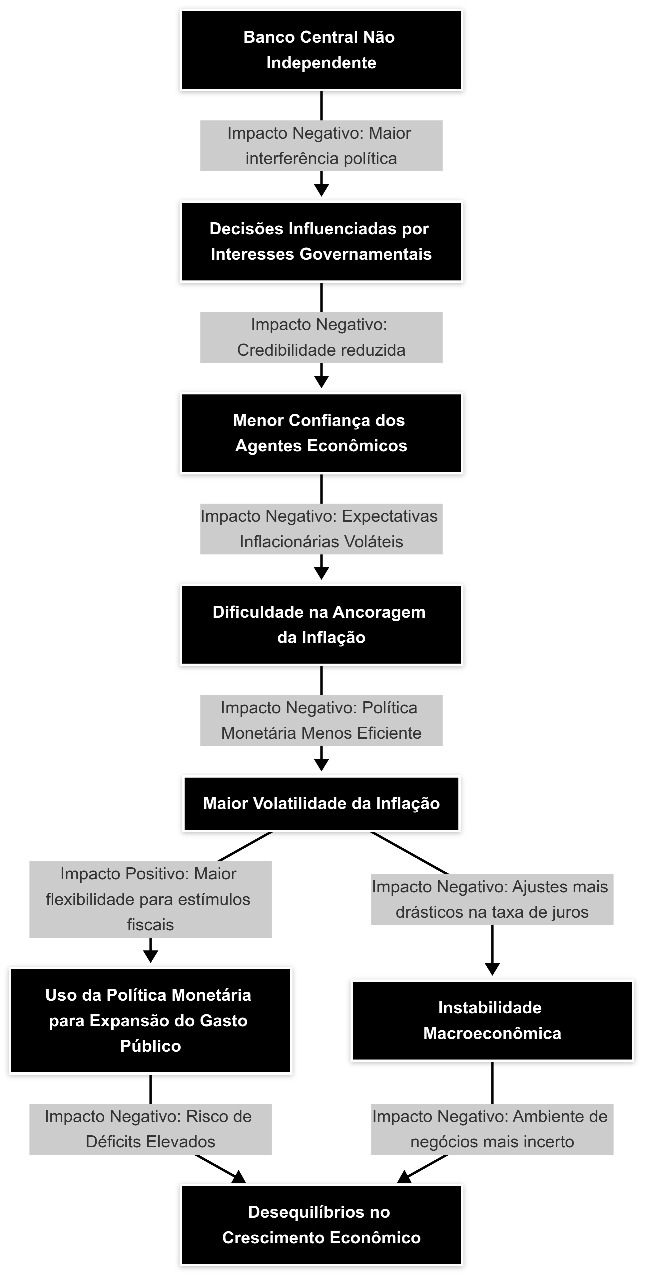
\includegraphics[width=\linewidth]{Imagens/m2i2.jpg}
        \caption{Banco Central Não Independente}
        \label{fig:bc_nao_independente}
    \end{subfigure}
    \caption{Cenários de condução da política monetária conforme grau de independência}
    \label{fig:comparacao_bc}
\end{figure}

Além disso, \cite{jacome2022} mostram que países da América Latina que reforçaram a independência de seus bancos centrais conseguiram reduzir episódios de hiperinflação.  Como ilustrado na Figura~\ref{fig:independencepays}, observa-se correlação negativa entre maior independência institucional e menores níveis de inflação na região.

\begin{figure}[H]
    \centering
    \caption{Evolução da independência do BC e inflação na América Latina}
    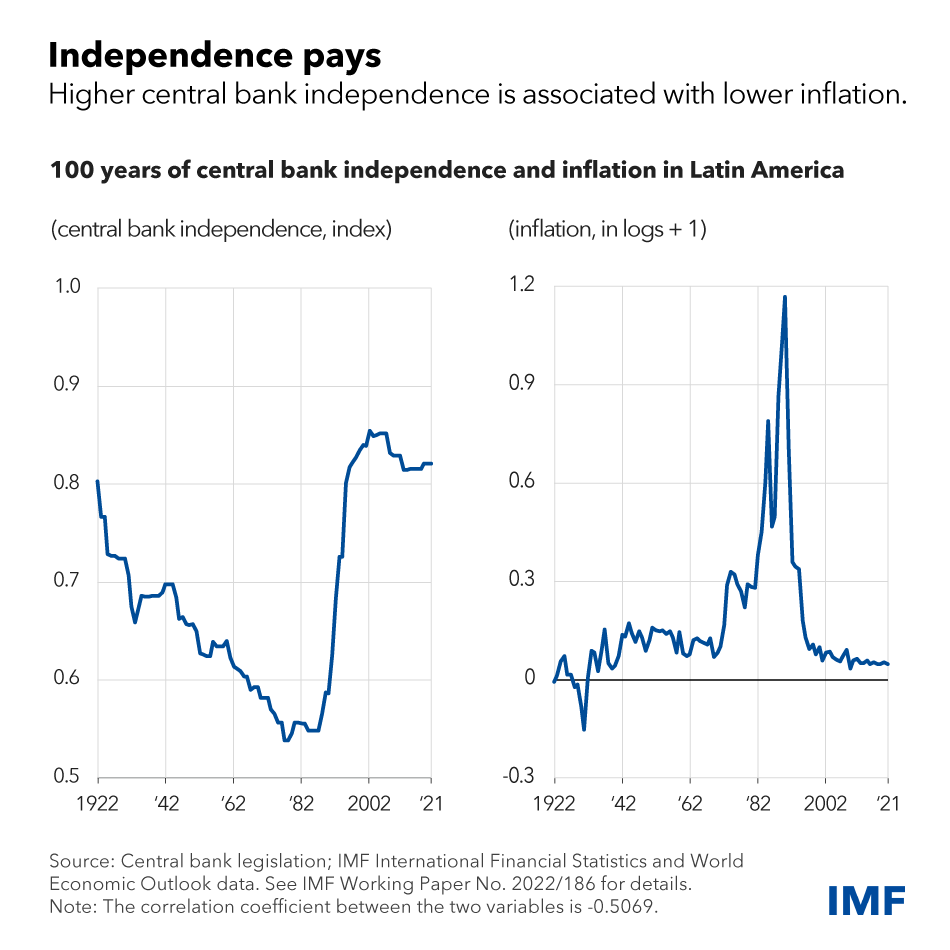
\includegraphics[width=.85\linewidth]{Imagens/m4i1.png}
    \label{fig:independencepays}
\end{figure}



\section{Referencial Teórico}

A teoria econômica oferece diferentes abordagens para entender o papel da autonomia do Banco Central. A literatura Novo-Keynesiana, por exemplo, destaca a importância da ancoragem das expectativas e da consistência temporal na condução de políticas eficazes. Nesse contexto, modelos com função de perda e regra de Taylor são amplamente utilizados para representar o comportamento da autoridade monetária.

\cite{adrian2024} desenvolvem um índice composto de independência que considera fatores legais e operacionais, incluindo mandatos, critérios de nomeação e autonomia financeira. Já \cite{jacome2022} analisam como o sucesso de reformas legais depende de arranjos institucionais que evitem interferências políticas recorrentes.

Por outro lado, \cite{acemoglu2008} argumentam que a independência do BC não garante, por si só, melhores resultados. Em contextos institucionais frágeis, a autonomia formal pode ser anulada por políticas fiscais desordenadas ou instabilidade política. Finalmente, \cite{unsal2023} enfatizam que a eficácia da autoridade monetária depende também de transparência, accountability e comunicação coerente.


\section{Modelo Econômico}

Com base na literatura revisada, o modelo adota uma estrutura Novo-Keynesiana com três componentes principais:

\subsection*{Curva de Phillips NK}
\[
\pi_t = \beta \, E_t[\pi_{t+1}] + \kappa \, (y_t - y_t^*) + \epsilon_t
\]

\subsection*{Equação IS}
\[
y_t - y_t^* = E_t[y_{t+1} - y_{t+1}^*] - \phi \, (i_t - E_t[\pi_{t+1}] - r_t^*) + \eta_t
\]

\subsection*{Regra de Taylor}
\[
i_t = \rho \, i_{t-1} + (1 - \rho)[r_t^* + \pi_t + \alpha(\pi_t - \pi^*) + \gamma(y_t - y_t^*)] + \nu_t
\]

\subsection*{Função de perda com independência}
\[
L = (y_t - y^T)^2 + \beta(CBI) \cdot (\pi_t - \pi^T)^2
\quad \text{com} \quad
\beta(CBI) = \beta_0 + \beta_1 \cdot CBI
\]

\subsection*{Potência da política monetária}
\[
\text{Potência} = \left| \frac{\partial \pi_t}{\partial r_t} \right| = \frac{\sigma}{\alpha \cdot \beta(CBI)}
\]

O modelo indica que quanto maior for a independência do BC (CBI), maior será o peso dado à estabilidade de preços, aumentando a potência da política monetária.


\section{Hipótese Econômica}

Com base no modelo proposto, a hipótese central do estudo é:

\begin{quote}
\textit{Quanto maior o grau de independência do Banco Central, maior será a potência da política monetária no controle da inflação.}
\end{quote}

Essa hipótese será testada empiricamente com base em:
\begin{itemize}
    \item Dados do Banco Central, IBGE e relatórios de mercado (ex: Boletim Focus);
    \item Índices de independência do BC desenvolvidos por \cite{adrian2024} e outros;
    \item Regressões com dados em painel comparando países da América Latina.
\end{itemize}


\section{Viabilidade Empírica}

A abordagem empírica considera o uso de:
\begin{itemize}
    \item Séries históricas de inflação, juros reais e expectativas inflacionárias;
    \item Indicadores de risco e credibilidade (CDS, prêmios de risco, etc.);
    \item Variáveis de controle como regime cambial, abertura comercial e choques externos.
\end{itemize}

Também será explorada a interação entre independência institucional e qualidade de governança, conforme sugerido por \cite{acemoglu2008}. O objetivo é verificar se a autonomia do BC é mais eficaz em contextos com \emph{checks and balances} robustos.


\section{Considerações Finais}

Este estudo propõe investigar como a independência do Banco Central afeta a eficácia da política monetária no Brasil. A partir de uma abordagem teórica consolidada e fundamentada na literatura empírica recente, pretende-se avaliar se a consolidação de uma autoridade monetária autônoma contribui para a estabilidade dos preços e redução de incertezas, promovendo um ambiente econômico mais previsível e favorável ao crescimento sustentável.


\section{Metodologia}
\lipsum[5]

\section{Análise e Resultados}
\lipsum[6-7]

\section{Conclusão}
\lipsum[8]

% Referências
\newpage
\printbibliography

\end{document}
